\newcommand{\N}{\mathbb{N}}
\newcommand{\Z}{\mathbb{Z}}
\newcommand{\R}{\mathbb{R}}

\newcommand{\parenth}[1]{\left(#1\right)}
\newcommand{\angl}[1]{\left\langle#1\right\rangle}
\newcommand{\floor}[1]{\left\lfloor#1\right\rfloor}
\newcommand{\ceil}[1]{\left\lceil#1\right\rceil}

\SetKw{Continue}{continue}
\SetKw{Break}{break}

\renewcommand*{\O}{\mathcal{O}}

\section{Introduction}
\label{sec:introduction}

Polyline simplification is the process of algorithmically reducing the number of points of a polyline while preserving its general shape up to a specified error parameter \(\varepsilon\). This technique is widely used in applications such as geographic information systems (GIS) to simplify map contours~\cite{algorithms_reduction_number_points_caricature}. To evaluate the quality of a simplification, distance functions between polylines are employed, with the Hausdorff and Fréchet distances being the most common. These distances can be applied either \emph{locally}, where each segment of the simplified polyline is compared with the corresponding subpolyline of the original, or \emph{globally}, where the entire simplification is compared to the original as a whole.

Local simplification has been extensively studied for both the Hausdorff and the Fréchet distances~\cite{polyline_simplification_under_the_local_frechet_distance_has_almost_quadratic_runtime_in_2d_storandtetal,computational_geometric_methods_for_polygonal_approximations_of_a_curve}. In contrast, global simplification has only recently gained attention. \citeauthor{on_optimal_polyline_simplification_using_the_hausdorff_and_frechet_distance} proposed a polynomial-time algorithm for global Fréchet simplification and proved that global Hausdorff simplification is NP-hard. Later, \citeauthor{polyline_simplification_has_cubic_complexity_bringmannetal} improved this result by developing a cubic-time algorithm and establishing conditional lower bounds for global Fréchet simplification as well as both local variants.

In this thesis, we provide a detailed discussion of these two algorithms, complete with examples. We explain every step, from solving the necessary equations to the full simplification algorithms, aiming to serve as a comprehensive guide for implementation. Furthermore, we present a wide array of optimizations to achieve better practical runtimes, including parallelization, compiler configuration, and hardware-specific considerations.

First, we define the terminology, definitions, and mathematical concepts used throughout this thesis in \cref{sec:preliminaries}. Then, in \cref{sec:preliminaries} we distinguish the more commonly used local variants from the global variants that are the focus of this work and derive simple properties to develop an intuition for working with the Fréchet distance.

Before discussing the simplification algorithms, we show how to solve various necessary equations in \cref{sec:equation_solving}, where we derive the formula for the Euclidean case and present algorithms for the Manhattan and Chebyshev cases. Following this, we explain the algorithm from \citeauthor{on_optimal_polyline_simplification_using_the_hausdorff_and_frechet_distance} for polyline simplification as well as the required algorithm from \citeauthor{computing_the_frechet_distance_between_two_polygonal_curves}. We visualize the algorithm with examples to build intuition and motivate applicable optimizations.

We continue more theoretically by proposing our implicit Fréchet framework in \cref{sec:implicit_polyline_simplification} and show how to transform current approaches, which we call explicit, into implicit ones using the examples of the previously discussed algorithms. The implicit approach relies on the fact that we never need to perform arithmetic on the solutions of equations from \cref{sec:equation_solving} but only comparisons. As a consequence, we show that in the Euclidean case, polyline simplification can be solved without square root and division operations while maintaining the same theoretical runtime. For general distances, the implicit approach is applicable and can potentially avoid the need to find roots of higher-order polynomials, though it requires solving problems in real algebraic geometry.

\cref{sec:cubic_algo} explains the algorithm from \citeauthor{polyline_simplification_has_cubic_complexity_bringmannetal} and the required cell reachability problem. Again, we explain the algorithms utilizing examples and mention practical considerations.

Having seen two algorithms to simplify a polyline for a single \(\varepsilon\), we present an algorithm that computes \emph{all} simplifications for a polyline in \cref{sec:simplification-queries}. For this, we determine the intervals in which the simplification size does not change. This allows the creation of a data structure that facilitates querying for simplifications given an \(\varepsilon\) in \(\O(\log n)\) time. The construction of this data structure relies on a deep analysis of the decisions made by the simplification algorithms. We show how to construct such a data structure in \(\Oh(n^4 \log n)\) time and \(\O(n^3)\) space. Interestingly, we show that this problem is much simpler in the Euclidean case than in the Manhattan or Chebyshev cases in multiple aspects, unlike the regular simplification algorithms which are largely distance-agnostic when treating the equation-solving algorithm as a black box.

In \cref{sec:global_imai_iri}, we address the problem of finding subcubic algorithms in two dimensions. In the local variants, this has been achieved by improving the algorithm from \citeauthor{computational_geometric_methods_for_polygonal_approximations_of_a_curve}. Using this as motivation, our goal is to adapt the same algorithm to the global variant to apply local techniques. The resulting algorithm is functionally equivalent to the one by \citeauthor{global_curve_simplification} but provides a more intuitive perspective on its underlying principles.

\cref{sec:evaluation} presents an extensive experimental evaluation of the implemented algorithms, which, to our knowledge, is the first for the global variants. We measure performance and simplification size while varying a multitude of parameters to demonstrate their effects.

Finally, we conclude with \cref{sec:discussion_conclusion} and mention possible future work.
 


\section{Related Work}
\label{sec:related_work}

In this section, we cover previous work on the topic of polyline simplification and how our work extends it. We focus here on works that apply to the thesis as a whole. More specific references relevant to individual areas are discussed in the subsequent sections.

Polyline simplification has been studied extensively due to its many applications. One of the oldest algorithms is the Douglas-Peucker algorithm \cite{algorithms_reduction_number_points_caricature}, proposed over fifty years ago, which is fast to compute but provides no optimality guarantees. To formalize an optimization objective, various distance measures between polylines have been studied, with the Hausdorff and Fréchet distances being the most widely used; both can be applied in numerous ways.

\citeauthor{computing_the_frechet_distance_between_two_polygonal_curves}~\cite{computing_the_frechet_distance_between_two_polygonal_curves} showed how to compute the Fréchet distance between two polylines and how to solve the corresponding decision problem. They also stated the problem of polyline simplification, which they called curve approximation, but did not provide a solution. The version they considered was minimization under the global Fréchet distance. Thus, this formulation of polyline simplification is at least 30 years old but has received relatively little attention.

The related local version, on the other hand, has been discussed in more detail. One of the most well-known locally optimal algorithms is by Imai and Iri \cite{computational_geometric_methods_for_polygonal_approximations_of_a_curve}, which has been the subject of numerous subsequent studies and improvements for various use cases.

The global version has only recently been studied in depth. \citeauthor{on_optimal_polyline_simplification_using_the_hausdorff_and_frechet_distance}~\cite{on_optimal_polyline_simplification_using_the_hausdorff_and_frechet_distance} showed that simplification under the global Fréchet distance can be solved in polynomial time, as well as showing that simplification under the global Hausdorff distance is NP-hard. However, their algorithm has a quintic runtime in the best case and a sextic runtime in the worst case. Although polynomial, this complexity makes it infeasible in practice, and it has, to our knowledge, not been implemented previously. In \cref{sec:algorithm_implementation}, we discuss this algorithm along with optimizations, practical considerations, and parallelization techniques that make it usable in practice.

\citeauthor{polyline_simplification_has_cubic_complexity_bringmannetal}~\cite{polyline_simplification_has_cubic_complexity_bringmannetal} improved upon the algorithm of \citeauthor{on_optimal_polyline_simplification_using_the_hausdorff_and_frechet_distance}, achieving cubic runtime. They further provided a conditional lower bound based on the \(\forall\forall\exists\)-Orthogonal Vector Hypothesis, ruling out subcubic runtime for various cases in high dimensions. For this algorithm, we also provide detailed explanations and practical optimizations to improve its performance in \cref{sec:cubic_algo}.



\section{Preliminaries}
\label{sec:preliminaries}

This section introduces the notation, conventions, and definitions used throughout this report.

We denote the set of natural numbers by \(\N\), which includes \(0\), and define \(\N_+ = \N \setminus\set{0}\) as the set of positive natural numbers.

\subsection{Polylines}
\label{ssec:polylines}

The central geometric object of our study is the \emph{polyline}, defined as follows:

\begin{definition}[Polyline]
  Let \(d\in \N_+\) and \(n \in \N\) be natural numbers, and let \(u_0, \dots, u_n \in \R^d\) be points in \(d\)-dimensional space.

  The sequence \(P = \angl{u_0, \dots, u_n}\) is a \(d\)-dimensional \emph{polyline} of length \(n\). It consists of \(n+1\) points connected by \(n\) line segments.
  \begin{itemize}
    \item We interpret \(P\) as a continuous function \(P:[0,n] \to \R^d\) such that \(P(i) = u_i\) for all \(i~\in~\set{0,~\dots,~n}\).
      Points in between integers are linearly interpolated: for \(t \in [0, 1]\) and \(i \in \set{0, \dots, n - 1}\), we set \(P(i + t) = (1- t)u_i + t u_{i+1} = u_i + t(u_{i+1} - u_i)\).
    \item We denote by \(P[t' \dots t]\) the subpolyline from parameter \(t' \in [0, n]\) to \(t \in [t', n]\). Formally,
			\[P[t' \dots t] = \angl{P(t'), P(\floor{t'} + 1),  P(\floor{t'} + 2), \dots, P(\ceil{t} - 1), P(t)}.\]
  \end{itemize}
\end{definition}

We denote the dimension by \(d\) throughout the report. Polylines are typically denoted by capital letters such as \(P\) and \(Q\). Single line segments are often denoted by \(e\).

The length of a polyline is typically denoted by \(n\), \(p\), or \(q\), where \(p\) and \(q\) are the lengths of \(P\) and \(Q\), respectively, and \(n\) is used when discussing a single polyline.

Following \citeauthor{polyline_simplification_has_cubic_complexity_bringmannetal}, we differentiate between \(\O\) and \(\Oh\) notation, where the latter hides polynomial factors in \(d\)\footnote{In this thesis, no exponential factors appear, so \(\Oh\) hides all factors depending on \(d\).}.

\subsection{Distances}
\label{ssec:distances}
We distinguish between distances between points and distances between polylines.

\begin{definition}[Distances]\label{def:point_distance}
  Let \(d \in \N_+\) and \(\ell \geq 1\).
  \begin{itemize}
    \item The \emph{unnormalized \(\ell\)-Minkowski distance} \(\delta'_\ell\) is defined as
      \[\delta'_\ell:\R^d \times \R^d \to \R_{\geq 0}, (u, v) \mapsto \sum_{i = 1}^d |u_i - v_i|^\ell.\]
    \item The \emph{(normalized) \(\ell\)-Minkowski distance} \(\delta_\ell\) is
      \[\delta_\ell:\R^d \times \R^d \to \R_{\geq 0}, (u, v) \mapsto \delta'_\ell(u, v)^{\frac1\ell} = \parenth{\sum_{i = 1}^d |u_i - v_i|^\ell}^{\frac1\ell}.\]
    \item The special case of \(\delta_2'\) is called the \emph{unnormalized Euclidean distance} and \(\delta_2\) the \emph{(normalized) Euclidean distance}.
    \item When \(\ell = 1\), the unnormalized and normalized versions coincide. We call \(\delta_1' = \delta_1\) the \emph{Manhattan distance}.
    \item We define the \emph{Chebyshev distance} \(\delta'_\infty = \delta_\infty\) as
      \[\delta_\infty:\R^d \times \R^d \to \R_{\geq 0}, (u, v) \mapsto \max_{i = 1, \dots, d} |u_i - v_i|.\]
    \item We define the auxiliary function \(\nu_\ell:\R_{\geq 0} \to \R_{\geq 0}\) as \(\nu_\ell(x) = x^\ell\) for \(\ell \neq \infty\) and \(\nu_\infty(x) = x\).
  \end{itemize}
  The subscript \(\ell\) is omitted when clear from context.
\end{definition}

The Euclidean distance (\(\ell = 2\)) is the most widely used metric. The Manhattan distance (\(\ell = 1\)) and Chebyshev distance (\(\ell = \infty\)) are computationally simpler, as they avoid roots.
Other Minkowski distances are less common due to numerical instability and lack of geometric interpretation. The unnormalized variants will later allow us to avoid explicit root computations in algorithms.

\begin{definition}[Fréchet Distance]\label{def:frechet}
  Let \(\delta\) be a normalized distance. The \emph{Fréchet distance} \(\delta^F\) between two polylines \(P\) and \(Q\) of lengths \(p\) and \(q\), respectively, is
	\[\delta^F(P, Q) = \inf_{\substack{f \in \mathcal{C}([0,1], [0, p]) \\ g \in \mathcal{C}([0,1], [0, q])}} \max_{t \in [0,1]}\delta(P(f(t)), Q(g(t))),\]
	where \(\mathcal{C}([a,b], [c,d])\) denotes the set of continuous, non-decreasing functions \(f\) mapping \([a,b]\) to \([c,d]\) with \(f(a) = c\) and \(f(b) = d\).
\end{definition}

\begin{definition}[Polyline Simplification]
	Given a polyline \(P\) of length \(n\), an error parameter \(\varepsilon > 0\), and a distance \(\delta\), the \emph{global Fréchet simplification problem} is to find a minimal subsequence \(Q\) of the vertices of \(P\) that includes the start point \(P(0)\) and the end point \(P(n)\), and satisfies \(\delta^F(P, Q) \leq \varepsilon\).
\end{definition}

This differs from \emph{local} simplification, where each line segment \(e = \overline{S(i)S(i+1)}\) of the simplification must satisfy \(\delta^F(e, P[j' \dots j]) \leq \varepsilon\) for its corresponding subpolyline. We focus on the global Fréchet case but cover the local one briefly in \cref{sec:polyline-simplification}.

We refer to a solution \(Q\) of the global Fréchet simplification problem as a \emph{polyline simplification}. Furthermore, any subsequence \(Q\) of \(P\) that includes \(P(0)\) and \(P(n)\) and satisfies \(\delta^F(P, Q) \leq \varepsilon\) will be referred to as a \emph{non-optimal simplification}; it meets all criteria except minimality.

\subsection{Properties of Distances}
All introduced distances are \emph{metrics} on \(\R^d\)~\cite{metric_spaces}:

\begin{definition}[Metric Spaces]\label{def:metric}
  Let \(X\) be a set and \(\delta:X\times X \to \R\). Then \(\delta\) is a \emph{metric} on \(X\) if for all \(a, b, c \in X\):
  \begin{itemize}
    \item \(\delta(a, b) \geq 0\) with equality if and only if \(a = b\), \hfill (Positivity)
    \item \(\delta(a, b) = \delta(b, a)\), and \hfill (Symmetry)
    \item \(\delta(a, c) \leq \delta(a, b) + \delta(b, c)\). \hfill (Triangle Inequality)
  \end{itemize}
  A set \(X\) together with a metric \(\delta\) is called a \emph{metric space}.
\end{definition}

\begin{observation}\label{obs:unnormalize}
  Let \(\ell \in [1, \infty]\), \(\varepsilon > 0\), and \(u, v \in \R^d\). Then
    \[\delta_\ell(u, v) \leq \varepsilon \iff \delta_\ell'(u, v) \leq \nu_\ell(\varepsilon).\]
\end{observation}

\begin{lemma}\label{lem:distance_properties}
	Let \(\delta\) be any Minkowski distance (including Chebyshev). For all \(u, v, w, x \in \R^d\), \(a \in \R\), and \(t \in [0, 1]\):
  \begin{enumerate}
		\item \(\delta(u, v) = \delta(u - w, v - w)\), \hfill (Translation Invariance)
		\item \(\delta(a u, a v) = |a| \delta(u, v)\), \hfill (Homogeneity)
		\item If \(\delta(u, w) \leq \varepsilon\) and \(\delta(v, w) \leq \varepsilon\), then \(\delta((1-t)u + tv, w) \leq \varepsilon\). \hfill (Convexity)
		\item \(\delta^F(\overline{uv}, \overline{wx}) \leq \varepsilon\) if and only if \(\delta(u, w) \leq \varepsilon\) and \(\delta(v, x) \leq \varepsilon\).
	\end{enumerate}
\end{lemma}

Property (3) implies that the set \(\set{u \mid \delta(u, v) \leq \varepsilon }\) is convex for fixed \(v \in \R^d\) and \(\varepsilon \geq 0\), motivating the name. Property (4) provides a simple characterization of the Fréchet distance between two line segments.

\begin{proof}
  \begin{enumerate}
    \item Follows directly from the definitions.
    \item Follows directly from the definitions.
		\item Assume \(\delta(u, w) \leq \varepsilon\) and \(\delta(v, w) \leq \varepsilon\). Let \(z = (1-t)u + tv\). Then,
			\begin{flalign*}
				\delta(z, w) &= \delta(z - w, 0) && \text{(Translation)} \\
        	&= \delta((1-t)(u-w) + t(v-w), 0) \\
					&\leq \delta((1-t)(u-w), 0) + \delta(t(v-w), 0) && \text{(Triangle Inequality)} \\
					&= (1-t)\delta(u-w, 0) + t\delta(v-w, 0) && \text{(Homogeneity)} \\
					&= (1-t)\delta(u, w) + t\delta(v, w) && \text{(Translation)} \\
					&\leq (1-t)\varepsilon + t\varepsilon = \varepsilon.
    \end{flalign*}
	\item (\(\Rightarrow\)) This direction follows because the reparameterizations \(f\) and \(g\) must satisfy \(f(0) = g(0) = 0\) and \(f(1) = g(1) = 1\), so the endpoints are matched at \(t=0\) and \(t=1\).

		(\(\Leftarrow\)) For the backward direction, consider the linear reparameterizations \(f(s) = s\) and \(g(s) = s\) for \(s \in [0,1]\). Then, for any \(s \in [0, 1]\),
    \begin{flalign*}
			\delta(P(f(s)), Q(g(s))) &= \delta((1-s)u + sv, (1-s)w + sx) \\
			&= \delta((1-s)(u-w) + s(v-x), 0) && \text{(Translation)} \\
			&\leq \delta((1-s)(u-w), 0) + \delta(s(v-x), 0) && \text{(Triangle Inequality)} \\
			&= (1-s)\delta(u, w) + s\delta(v, x) && \text{(Homogeneity and Translation)} \\
			&\leq (1-s)\varepsilon + s\varepsilon = \varepsilon.
    \end{flalign*}
		Since the maximum over \(s \in [0,1]\) is at most \(\varepsilon\), the Fréchet distance is at most \(\varepsilon\).
  \end{enumerate}
\end{proof}


\section{Equation Solving}
\label{sec:equation_solving}
Before delving into the core simplification algorithms, we must address a fundamental subproblem: the \emph{line segment intersection problem}.

\begin{definition}[Line Segment Intersection Problem]
  Let \(e = \overline{e_1e_2}\) be a \(d\)-dimensional line segment, \(u \in \R^d\) a point, \(\varepsilon > 0\), and \(\delta\) a distance function. The \emph{line segment intersection problem} is to determine the set
	\[\set{t \in [0, 1] \mid \delta(e_1 + t(e_2 - e_1), u) \leq \varepsilon},\]
	where \(t\) is the parameter along the line segment \(e\).

  Geometrically, this corresponds to the intersection of the line segment \(e\) and the set of points within distance \(\varepsilon\) of \(u\), \(\set{x \in \R^d \mid \delta(x, u) \leq \varepsilon}\).
\end{definition}

\begin{observation}
	For any \(\ell \in [1, \infty]\), the solution set to the line segment intersection problem using the distance \(\delta_\ell\) is convex. Therefore, it can be expressed as a single (possibly empty) closed interval \(I \subseteq [0, 1]\), identifiable by its left and right boundaries.
\end{observation}

\begin{proof}
  This follows directly from the convexity property in \cref{lem:distance_properties} and the fact that both the line segment and the \(\varepsilon\)-ball are convex sets.
\end{proof}

This convexity simplifies the problem to finding the interval's boundaries. We do this by solving the equation
\begin{equation}
  \delta(u + t \cdot (v - u), w) = \varepsilon \label{eq:eq_solve_main}
\end{equation}
for \(t \in \R\), given fixed vectors \(u, v, w \in \R^d\) and \(\varepsilon > 0\). This equation finds points on the entire line through \(u\) and \(v\) that are at distance \(\varepsilon\) from \(w\).

Let \(\hat{t}_0\) and \(\hat{t}_1\) be the smallest and largest solutions to \cref{eq:eq_solve_main}, respectively. These may lie outside the interval \([0,1]\), coincide (a single point solution), or may not exist. The actual solution interval for the line segment \(\overline{uv}\) is \([\hat t_0, \hat t_1] \cap [0, 1]\). We define the modified solutions \(\hat{t}_0'\) and \(\hat{t}_1'\) that account for the segment boundaries:

\begin{equation}
  \hat{t}_0' \coloneq \begin{cases}
    0 & \text{if } \hat{t}_0 < 0 \text{ and } \hat{t}_1 \geq 0,\\
    \hat{t}_0 & \text{if } \hat{t}_0 \in [0, 1],\\
    \infty &\text{otherwise},
  \end{cases}
	\quad
  \hat{t}_1' \coloneq \begin{cases}
    1 & \text{if } \hat{t}_1 > 1 \text{ and } \hat{t}_0 \leq 1,\\
    \hat{t}_1 & \text{if } \hat{t}_1 \in [0, 1],\\
    \infty &\text{otherwise}.
  \end{cases}
\end{equation}

The \(\infty\) value indicates an empty intersection. \Cref{fig:solution_kinds} illustrates these cases. For a line segment \(\overline{uv}\) and point \(w\), we denote the relevant solutions as \(\hat t_0'(\overline{uv}, w)\) and \(\hat t_1'(\overline{uv}, w)\); the parameter \(\varepsilon\) is omitted as it is fixed contextually.

\begin{figure}
    \centering
    % First row of subfigures
    \begin{subfigure}[t]{0.3\textwidth}
      \includegraphics{tikz-fig/solution-kinds-1.pdf}
      \caption{\(\hat t_0 < 0 < \hat t_1 < 1\) \\
        \(\hat t_0' = 0, \hat t_1' = \hat t_1\)}
    \end{subfigure}
    \hfill
    \begin{subfigure}[t]{0.3\textwidth}
      \includegraphics{tikz-fig/solution-kinds-2.pdf}
      \caption{\(0 < \hat t_0 < \hat t_1 < 1\) \\
        \(\hat t_0' = \hat t_0, \hat t_1' = \hat t_1\)}
    \end{subfigure}
    \hfill
    \begin{subfigure}[t]{0.3\textwidth}
      \includegraphics{tikz-fig/solution-kinds-3.pdf}
      \caption{\(0 < \hat t_0 < 1 < \hat t_1 \) \\
        \(\hat t_0' = \hat t_0, \hat t_1' = 1\)}
    \end{subfigure}

    % Second row of subfigures
    \begin{subfigure}[t]{0.3\textwidth}
      \includegraphics{tikz-fig/solution-kinds-4.pdf}
      \caption{\(\hat t_0 < \hat t_1 < 0\) \\
        \(\hat t_0' = \hat t_1' = \infty\)}
    \end{subfigure}
    \hfill
    \begin{subfigure}[t]{0.3\textwidth}
      \includegraphics{tikz-fig/solution-kinds-5.pdf}
      \caption{\(\hat t_0 < 0 < 1 < \hat t_1\) \\
        \(\hat t_0' = 0, \hat t_1' = 1\)}
    \end{subfigure}
    \hfill
    \begin{subfigure}[t]{0.3\textwidth}
      \includegraphics{tikz-fig/solution-kinds-6.pdf}
      \caption{\(1 < \hat t_0 < \hat t_1\) \\
        \(\hat t_0' =  \hat t_1' = \infty\)}
    \end{subfigure}

    % Third row of subfigures (centered)
    \begin{subfigure}[t]{0.3\textwidth}
      \includegraphics{tikz-fig/solution-kinds-7.pdf}
      \caption{\(\hat t_0, \hat t_1\) do not exist \\
        \(\hat t_0' = \hat t_1' = \infty\)}
    \end{subfigure}
    \caption{The different kinds of solutions. Note that we associate \(0\) with \(u\), \(1\) with \(v\), and \(t\) with \((1-t)u + tv\)}
    \label{fig:solution_kinds}
\end{figure}

Solving \cref{eq:eq_solve_main} generally involves finding roots of polynomials. For Minkowski distances \(\delta_\ell\) with \(\ell > 4\), no closed-form solution exists due to the Abel-Ruffini theorem. We now derive explicit solutions for the Euclidean, Manhattan, and Chebyshev distances.

\subsection{Euclidean Distance}
\label{ssec:eq_euclidean_distance}
For the Euclidean distance \(\delta_2\), \cref{eq:eq_solve_main} becomes:
\begin{align*}
  \| (u - w) + t(v - u) \|_2 &= \varepsilon \\
  \| (u - w) + t(v - u) \|_2^2 &= \varepsilon^2.
\end{align*}
Expanding the squared norm yields a quadratic equation in \(t\):
\begin{align*}
  \| u - w \|_2^2 + 2\braket{u - w | v - u} t + \| v - u \|_2^2 t^2 &= \varepsilon^2.
\end{align*}
Define the coefficients:
\begin{align*}
	\alpha_0 &= \delta(u,w)^2 - \varepsilon^2, \\
	\alpha_1 &= \braket{u - w | v - u}, \\
	\alpha_2 &= \delta(v, u)^2.
\end{align*}
The equation is \(\alpha_0 + 2\alpha_1 t + \alpha_2 t^2 = 0\). The solutions are:
\begin{equation}
	\hat t_{0,1} = \frac{-\alpha_1 \pm \sqrt{\alpha_1^2 - \alpha_0\alpha_2}}{\alpha_2}.\label{eq:sol_explicit_euclidean}
\end{equation}
If the discriminant \(\alpha_1^2 - \alpha_0\alpha_2\) is negative, there are no real solutions. Otherwise, \(\hat{t}_0\) and \(\hat{t}_1\) are the smaller and larger root, respectively. Here, we use Dirac notation for the inner product as \(\langle \cdot , \cdot \rangle\) denotes a polyline of length \(1\).

\subsection{Manhattan Distance}
\label{ssec:eq_manhattan_distance}
For the Manhattan distance \(\delta_1\), the equation is:
\begin{equation}
  \sum_{i=1}^d |u_i - w_i + t (v_i - u_i)| = \varepsilon. \label{eq:solve_manhattan}
\end{equation}

We use the following invariance property:
\begin{observation}\label{obs:permute-coordinates}
	Let \(\sigma\) be a permutation of \(\set{1, \dots, d}\). For any \(\ell \in [1, \infty]\), \(\delta_\ell(u, v) = \delta_\ell(\sigma(u), \sigma(v))\), where \(\sigma(u)\) denotes permuting the coordinates of \(u\).
\end{observation}

Each term \(|u_i - w_i + t (v_i - u_i)|\) is a piecewise linear function in \(t\), with a breakpoint at \(t_i = (w_i - u_i)/(v_i - u_i)\), where the expression inside the absolute value is zero. For a fixed \(t\), the sum becomes linear.

Let \(\sigma\) be a permutation that sorts the breakpoints: \(t_{\sigma(1)} \leq t_{\sigma(2)} \leq \dots \leq t_{\sigma(d)}\). By \cref{obs:permute-coordinates}, we can analyze the problem in this sorted order. In each interval between consecutive breakpoints, the equation is linear and can be solved for \(t\). We check if the solution lies within the current interval.

A na\"ive sweep-line algorithm would sort the breakpoints (\(\O(d \log d)\)) and check each of the \(d+1\) intervals in \(\O(d)\) time, leading to \(\O(d^2)\) total time. However, because only one term changes sign between intervals, the linear expression can be updated in constant time, reducing the total time to \(\O(d \log d)\).

We handle edge cases as follows:
\begin{itemize}
	\item Coinciding breakpoints require no special treatment; the function remains contiunous.
	\item If \(v_i = u_i\), the term is constant \(|u_i - w_i|\) and is subtracted from \(\varepsilon\).
\end{itemize}

\begin{algorithm}[ht]
  \DontPrintSemicolon
  \KwData{Vectors \(u, v, w \in \R^d\), \(\varepsilon > 0\)}
  \KwResult{Solution to \cref{eq:solve_manhattan}}
  \BlankLine
  \(global\_slope \gets 0, global\_offset \gets 0\) \;
  \(events \gets Array(d)\) \;
  \For{\(i = 1\) \KwTo \(d\)}{
    \(slope \gets v_i - u_i, offset \gets u_i - w_i\)\;
    \If{\(slope < 0\)}{
      \(slope \gets -slope, offset \gets -offset\)
    } \ElseIf{\(slope = 0\)}{
      \(\varepsilon \gets \varepsilon - |offset|\)\;
      \Continue
    }
    \(zero \gets - \frac{offset}{slope}\)\;
    \If{\(zero \leq 0\)}{
      \(global\_offset \gets global\_offset + offset\)\;
      \(global\_slope \gets global\_slope + slope\)\;
      \Continue
    }
    \(global\_offset \gets global\_offset - offset\)\;
    \(global\_slope \gets global\_slope - slope\)\;
    \If{\(zero \geq 1\)}{
      \Continue
    }
    \(events.append((zero, slope, offset))\)\;
  }
  Sort \(events\) by their \(zero\) component\;
  \(start \gets 0\)\;
  \For{\((zero, slope, offset) \in events\)}{
    Test if solution \(\frac{\varepsilon - global\_offset}{global\_slope} \in [start, zero]\) and report it if so\;
    \(global\_offset \gets global\_offset + 2offset\)\;
    \(global\_slope \gets global\_slope + 2slope\)\;
    \(start \gets zero\)
  }
  Test if solution \(\frac{\varepsilon - global\_offset}{global\_slope} \in [start, 1]\) and report it if so\;

  \caption{manhattan\_solver(\(u, v, w, \varepsilon\))}
  \label{algo:solve_manhattan}
\end{algorithm}

\paragraph{Linear-Time Variant using Quickselect}
The runtime can be reduced to expected \(\O(d)\) time by noting that a full sort is unnecessary; we only need the breakpoints that bound the potential solutions. This can be achieved with a modified Quickselect algorithm.

We represent each coordinate's contribution as a pair \((a, b)\) corresponding to \(|a + b t|\). The zero of this term is at \(t = -a/b\). We define an ordering between pairs \((a, b)\) and \((c, d)\) based on their zeros: \((a, b) < (c, d) \iff a d > b c\). This comparison is division-free and numerically stable.

The algorithm proceeds as follows:
\begin{enumerate}
	\item Start with artificial left and right boundaries representing \(t = -\infty\) and \(t = \infty\).
	\item Select a pivot pair and partition the other pairs based on their zero relative to the pivot's zero.
	\item Merge all pairs with the same zero into the pivot.
	\item Evaluate the Manhattan distance at the pivot's zero using the current global linear function (maintained incrementally).
	\item Exploiting the convexity of the distance function, determine whether a solution exists to the left, right, or on both sides of the pivot, and recurse on the relevant partition.
\end{enumerate}

This method finds the solutions in expected \(\O(d)\) time. A deterministic \(\O(d)\) worst-case time is possible using median-of-medians for pivot selection.

\subsection{Chebyshev Distance}
\label{ssec:eq_chebyshev_distance}
For the Chebyshev distance \(\delta_\infty\), the equation is:
\begin{equation}
  \max_{i = 1,\dots, d} |u_i - w_i + t(v_i - u_i)| = \varepsilon.\label{eq:solve_chebyshev}
\end{equation}

\paragraph{Na\"ive Approach}
A simple method considers all \(2d\) candidate expressions (positive and negative branches of each absolute value). For each candidate \(t\) where a specific term might achieve the maximum, we check if it indeed equals \(\varepsilon\) and is maximal. This leads to an \(\O(d^2)\) algorithm, practical for small \(d\).

\paragraph{Geometric Approach}
Each term \(|u_i - w_i + t(v_i - u_i)|\) is linear in \(t\). The problem reduces to finding where the upper envelope of these \(2d\) lines reaches height \(\varepsilon\) over \(t \in [0,1]\). A sweep-line algorithm, inspired by Bentley-Ottmann~\cite{computational_geometry}, maintains the upper envelope using a doubly-linked list and a priority queue for intersections. This runs in \(\O(d \log d)\) time. Pseudocode is provided in \cref{algo:solve_chebyshev_init,algo:solve_chebyshev}, and an example is illustrated in \cref{fig:chebyshev_algo}.

\begin{figure}
  \centering
  \begin{subfigure}[t]{0.3\textwidth}
		\includegraphics{tikz-fig/chebyshev-algo-1.pdf}
    \caption{All candidate lines}
  \end{subfigure}
  \begin{subfigure}[t]{0.3\textwidth}
    \includegraphics{tikz-fig/chebyshev-algo-2.pdf}
    \caption{Lines that are not fully negative}
  \end{subfigure}
  \begin{subfigure}[t]{0.3\textwidth}
    \includegraphics{tikz-fig/chebyshev-algo-3.pdf}
    \caption{Lines that are not fully below another line}
  \end{subfigure}\\
  \begin{subfigure}[t]{0.3\textwidth}
    \includegraphics{tikz-fig/chebyshev-algo-4.pdf}
    \caption{Find next intersection. Here between topmost line so check for solution.}
  \end{subfigure}
  \begin{subfigure}[t]{0.3\textwidth}
    \includegraphics{tikz-fig/chebyshev-algo-5.pdf}
    \caption{Find next intersection. No solution found}
  \end{subfigure}
  \begin{subfigure}[t]{0.3\textwidth}
    \includegraphics{tikz-fig/chebyshev-algo-6.pdf}
    \caption{Check final line for an intersection}
  \end{subfigure}
  \caption{Line representation for solving \(\delta_\infty((0,0,0) + t(-2,0,3), (-2,-1,1)) = 1.5\).}
  \label{fig:chebyshev_algo}
\end{figure}

\begin{algorithm}[ht]
  \DontPrintSemicolon
  \KwData{vectors \(u, v, w \in \R^d\), \(\varepsilon > 0\)}
  \BlankLine
  \(candidates \gets \set{(2i, u_i - w_i, v_i - u_i), (2i+1, w_i - u_i, u_i - v_i) | i = 0, \dots, d - 1}\) \;
  \(queue \gets PriorityQueue()\) \;
  \(list \gets Array(|candidates|)\) \;
  sort candidates according to second component descendingly,
  in case of ties use the third component as tie breaker descendingly \;
  \(PREV \gets 0, NEXT \gets 1\) \tcp{constants for readability}
  \(curr \gets -1\) \;
  \For{\((i, a, b) \in candidates\)}{
    \If{\(curr = -1\)} {
      \(curr \gets i, a' \gets a, b' \gets b\)\;
      \(list[curr] \gets (-1, -1, a, b)\) \;
      \Continue
    }

    \If{\( a' + b' \geq a + b\)}{
      \Continue \tcp{new line fully below current line so never maximum}
    }

    \(list[curr][NEXT] \gets i, list[i] \gets (curr, -1, a, b)\) \;
    \(intersection \gets \frac{a' - a}{b - b'}\) \tcp{always in \([0,1]\)}
    \(queue.insert\_with\_priority((curr, i), intersection)\) \;
    \(curr \gets i, a' \gets a, b' \gets b\) \;
  }

  \caption{chebyshev\_solver\_initialization(\(u, v, w\))}
  \label{algo:solve_chebyshev_init}
\end{algorithm}

\begin{algorithm}[ht]
  \DontPrintSemicolon
  \KwData{vectors \(u, v, w \in \R^d\), \(\varepsilon > 0\)}
  \KwResult{Solution to \cref{eq:solve_chebyshev}}
  \BlankLine
  \(chebyshev\_solver\_initialization(u, v, w)\) \;
  \(last\_intersection \gets 0\) \;
  \While{\(\lnot queue.empty()\)}{
    \((i, j), intersection \gets queue.poll()\) \;
    \If{\(list[i][PREV] = -1 \lor list[j][PREV] = -1\)}{
      \Continue \tcp{One of the lines already removed, no intersection}
    }
    \If{\(i = HEAD\)}{
      \(HEAD \gets j\) \;
      \(\_, \_, a, b \gets list[i]\) \;
      \If{\(b = 0\)}{
        \If{\(a = \varepsilon\) }{
          Mark \(last\_intersection\) as earliest solution or \(intersection\) as last solution \;
        }
        \(last\_intersection \gets intersection\) \;
        \Continue
      }
      \(solution \gets \frac{\varepsilon - a}{b}\) \;
      Mark \(solution\) as earliest or last solution if \(solution \in [last\_intersection, intersection]\) \;
      \(last\_intersection \gets intersection\) \;
      \Continue
    }
    \(before_i \gets list[i][PREV]\) \;
    \(list[before_i][NEXT] \gets j, list[j][PREV] \gets before_i\) \;
    \(list[i][PREV] \gets -1\) \tcp{mark as removed}
    \(last\_intersection \gets intersection\) \;
    \If{\(before_i \neq HEAD\)}{
      \(\_, \_, a, b \gets list[j]\) \;
      \(\_, \_, a', b' \gets list[before_i]\) \;
      \(intersection \gets \frac{a' - a}{b - b'}\) \tcp{also in \([0,1]\)}
      \(queue.insert\_with\_priority((before_i, j), intersection)\) \;
    }
  }
  Check for solution in \([last\_intersection, 1]\) \;

  \caption{chebyshev\_solver(\(u, v, w, \varepsilon\))}
  \label{algo:solve_chebyshev}
\end{algorithm}

\paragraph{Algebraic Approach}
A simpler and more efficient \(\O(d)\) method exists. Observe that:
	\[\max_{i} |a_i + t b_i| = \varepsilon \iff \forall i: |a_i + t b_i| \leq \varepsilon \ \land\ \exists i: |a_i + t b_i| = \varepsilon.\]
Each inequality \(|a_i + t b_i| \leq \varepsilon\) defines an interval for \(t\). If \(b_i > 0\), the interval is \([(-\varepsilon - a_i)/b_i, (\varepsilon - a_i)/b_i]\). If \(b_i < 0\), we flip signs to get an equivalent interval. If \(b_i = 0\), the inequality becomes \(|a_i| \leq \varepsilon\); if false, there is no solution.

The solution set is the intersection of these intervals, computable in \(\O(d)\) time by tracking the maximum left boundary and minimum right boundary. We then check if any term equals \(\varepsilon\) within this interval.

\paragraph{Summary}
We presented three methods for the Chebyshev case: a na\"ive \(\O(d^2)\) method, a geometric \(\O(d \log d)\) method, and an algebraic \(\O(d)\) method. The linear-time algebraic method is preferred for its simplicity and efficiency.

As a final note on the practical implementation of these equation-solving algorithms, we emphasize the need to account for floating-point inaccuracies. Special care must be taken to ensure that essential solutions are not lost. For instance, when computing the solution interval for a line segment relative to one of its endpoints, the result should never be an empty interval due solely to numerical error.


\section{Algorithm \& Implementation}
\label{sec:algorithm_implementation}


\subsection{Equation Solving}
\label{subsec:equation_solving}
For the following algorithms we need to solve equations involving distance functions \(\delta\). More specifically, we want to solve the following equation 
\begin{equation}
  \delta(u + t \cdot (v - u), w) = \varepsilon \label{eq:eq_solve_main}
\end{equation}
for arbitrary, fixed vectors \(u, v, w \in \R^d\) and fixed \(\varepsilon \in \R_{>0}\) for the variable \(t \in \R\) or determine that there is no such solution. This corresponds to the points the lie on the line segment \(e = \overline{uv}\) that have distance \(\varepsilon\) from \(w\) as each point on \(e\) is of the form \(u + t(v-u)\). 

By the third property of \cref{lem:distance_properties} we know that \(\set{x \in \R^d \mid \delta(x, w) \leq \varepsilon}\) is a convex set of points thus the set \(\set{t \in \R \mid \delta(u + t(v-u), w) \leq \varepsilon}\) is also convex and thus an interval \([a, b]\). Thus we only need to find the first and last solution to this equation even if there are more (which may only happen for the Chebyshev and Manhattan distance). We label the smallest solution \(\hat{t}_0\) and largest solution \(\hat{t}_1\). Those two solutions may be the same, i.e, the interval collapses to a single point, or may not exist at all, meaning the interval is empty.

For our use cases we do not need the actual solutions \(\hat{t}_0\) and \(\hat{t}_1\) but modified solutions \(\hat{t}_0'\) and \(\hat{t}_1'\) which are defined as 
\begin{equation}
  \hat{t}_0' \coloneq \begin{cases}
    0 & \textrm{ if } \hat{t}_0 < 0 \textrm{ and } \hat{t}_1 \geq 0\\
    \hat{t}_0 & \textrm{ if } \hat{t}_0 \in [0, 1]\\
    \infty &\textrm{ otherwise }
  \end{cases}\\
  \hat{t}_1' \coloneq \begin{cases}
    1 & \textrm{ if } \hat{t}_1 > 1 \textrm{ and } \hat{t}_0 \leq 1\\
    \hat{t}_1 & \textrm{ if } \hat{t}_1 \in [0, 1]\\
    \infty &\textrm{ otherwise }
  \end{cases},
\end{equation}
where the \emph{otherwise} case also includes the case of there being no solution to \cref{eq:eq_solve_main}. This corresponds to the smallest and largest point in the modified interval \([\hat t_0, \hat t_1] \cap [0, 1]\). How this can affect the solutions can be seen in \cref{fig:solution_kinds}.
For a line segment \(\overline{uv}\) and a point \(w\) we denote \(\hat t_0'(\overline{uv}, w)\) and \(\hat t_1'(\overline{uv}, w)\) to be the respective modified solutions for the given line segment and point. We do not include \(\varepsilon\) in that notation as it is fixed throughout all algorithms and thus needs to disambiguation.

\begin{figure}
    \centering
    % First row of subfigures
    \begin{subfigure}[b]{0.3\textwidth}
        \centering
        \begin{tikzpicture}
            % Define points
            \coordinate (u)  at (2,0.5);
            \coordinate (u0) at (0,0);
            \coordinate (v) at (4,1);
            \coordinate (w) at (2,0);

            % Draw the line segment from u to v
            \draw[thick] (u) -- (v);

            \draw[thick] (w) circle (1);

            % Find intersection points between the line and the circle
            \path[name path=line] (u0) -- (v);
            \path[name path=circle] (w) circle (1);
            \path[name intersections={of=line and circle, by={t1,t0}}];

            % Label intersection points
            \node[circle,fill,color=red,inner sep=1pt,label={[text=red, below]:\(u=\hat t_0'\)}] at (u) [] {}; 
            \node[circle,fill,color=blue,inner sep=1pt,label={[text=blue]-90:\(v\)}] at (v) [] {}; 
            \node[circle,fill,color=blue,inner sep=1pt,label={[text=blue]-90:\(w\)}] at (w) [] {}; 

            \node[circle,fill,color=red,inner sep=1pt,label={[text=red, above left]:\(\hat t_0\)}] at (t0) [] {}; 
            \node[circle,fill,color=red,inner sep=1pt,label={[text=red, above]:\(\hat t_1=\hat t_1'\)}] at (t1) [] {}; 

            % Draw dotted extensions of the line segment
            \draw[dotted] (u0) -- (u);
            %\draw[dotted] (v) -- ($(v)!-1.5!(u)$);
        \end{tikzpicture}
      \caption{\(\hat t_0 < 0 < \hat t_1 < 1\) \\ \(\hat t_0' = 0, \hat t_1' = \hat t_1\)}
    \end{subfigure}
    \hfill
    \begin{subfigure}[b]{0.3\textwidth}
        \centering
        \begin{tikzpicture}
            % Define points
            \coordinate (u) at (0,0);
            \coordinate (v) at (4,1);
            \coordinate (w) at (2,0);

            % Draw the line segment from u to v
            \draw[thick] (u) -- (v);

            \draw[thick] (w) circle (1);

            % Find intersection points between the line and the circle
            \path[name path=line] (u) -- (v);
            \path[name path=circle] (w) circle (1);
            \path[name intersections={of=line and circle, by={t1,t0}}];

            % Label intersection points
            \node[circle,fill,color=blue,inner sep=1pt,label={[text=blue]-90:\(u\)}] at (u) [] {}; 
            \node[circle,fill,color=blue,inner sep=1pt,label={[text=blue]-90:\(v\)}] at (v) [] {}; 
            \node[circle,fill,color=blue,inner sep=1pt,label={[text=blue]-90:\(w\)}] at (w) [] {}; 

            \node[circle,fill,color=red,inner sep=1pt,label={[text=red, above left]:\(\hat t_0=\hat t_0'\)}] at (t0) [] {}; 
            \node[circle,fill,color=red,inner sep=1pt,label={[text=red, above]:\(\hat t_1=\hat t_1'\)}] at (t1) [] {}; 

            % Draw dotted extensions of the line segment
            %\draw[dotted] ($(u)!-1.5!(v)$) -- (u);
            %\draw[dotted] (v) -- ($(v)!-1.5!(u)$);
        \end{tikzpicture}
        \caption{\(0 < \hat t_0 < \hat t_1 < 1\)\\ \(\hat t_0' = \hat t_0, \hat t_1' = \hat t_1\)}
    \end{subfigure}
    \hfill
    \begin{subfigure}[b]{0.3\textwidth}
        \centering
        \begin{tikzpicture}
            % Define points
            \coordinate (v)  at (2,0.5);
            \coordinate (u) at (0,0);
            \coordinate (v0) at (4,1);
            \coordinate (w) at (2,0);

            % Draw the line segment from u to v
            \draw[thick] (u) -- (v);

            \draw[thick] (w) circle (1);

            % Find intersection points between the line and the circle
            \path[name path=line] (u) -- (v0);
            \path[name path=circle] (w) circle (1);
            \path[name intersections={of=line and circle, by={t1,t0}}];

            % Label intersection points
            \node[circle,fill,color=blue,inner sep=1pt,label={[text=blue, below]:\(u\)}] at (u) [] {}; 
            \node[circle,fill,color=red,inner sep=1pt,label={[text=red, below]:\(v=\hat t_1'\)}] at (v) [] {}; 
            \node[circle,fill,color=blue,inner sep=1pt,label={[text=blue]-90:\(w\)}] at (w) [] {}; 

            \node[circle,fill,color=red,inner sep=1pt,label={[text=red, above left]:\(\hat t_0=\hat t_0'\)}] at (t0) [] {}; 
            \node[circle,fill,color=red,inner sep=1pt,label={[text=red, above]:\(\hat t_1\)}] at (t1) [] {}; 

            % Draw dotted extensions of the line segment
            \draw[dotted] (v) -- (v0);
            %\draw[dotted] (v) -- ($(v)!-1.5!(u)$);
        \end{tikzpicture}
      \caption{\(0 < \hat t_0 < 1 < \hat t_1 \) \\ \(\hat t_0' = \hat t_0, \hat t_1' = 1\)}
    \end{subfigure}

    % Second row of subfigures
    \begin{subfigure}[b]{0.3\textwidth}
        \centering
        \begin{tikzpicture}
            % Define points
            \coordinate (u) at (0,0);
            \coordinate (v0) at (4,1);
            \coordinate (v) at (2,0.5);
            \coordinate (w) at (3,0);

            % Draw the line segment from u to v
            \draw[thick] (u) -- (v);

            \draw[thick] (w) circle (1);

            % Find intersection points between the line and the circle
            \path[name path=line] (u) -- (v0);
            \path[name path=circle] (w) circle (1);
            \path[name intersections={of=line and circle, by={t1,t0}}];

            % Label intersection points
            \node[circle,fill,color=blue,inner sep=1pt,label={[text=blue]-90:\(u\)}] at (u) [] {}; 
            \node[circle,fill,color=blue,inner sep=1pt,label={[text=blue, above]:\(v\)}] at (v) [] {}; 
            \node[circle,fill,color=blue,inner sep=1pt,label={[text=blue]-90:\(w\)}] at (w) [] {}; 

            \node[circle,fill,color=red,inner sep=1pt,label={[text=red, below right]:\(\hat t_0\)}] at (t0) [] {}; 
            \node[circle,fill,color=red,inner sep=1pt,label={[text=red, above]:\(\hat t_1\)}] at (t1) [] {}; 

            % Draw dotted extensions of the line segment
            \draw[dotted] (v) -- (v0);
            %\draw[dotted] (v) -- ($(v)!-1.5!(u)$);
        \end{tikzpicture}
        \caption{\(\hat t_0 < \hat t_1 < 0\)\\ \(\hat t_0' = \hat t_1' = \infty\)}
    \end{subfigure}
    \hfill
    \begin{subfigure}[b]{0.3\textwidth}
        \centering
        \begin{tikzpicture}
            % Define points
            \coordinate (u0) at (-1.5,-0.5);
            \coordinate (u) at (-0.75,-0.125);
            \coordinate (v) at (0.5,0.5);
            \coordinate (v0) at (1.5,1);
            \coordinate (w) at (0,0);

            % Draw the line segment from u to v
            \draw[thick] (u) -- (v);

            \draw[thick] (w) circle (1);

            % Find intersection points between the line and the circle
            \path[name path=line] (u0) -- (v0);
            \path[name path=circle] (w) circle (1);
            \path[name intersections={of=line and circle, by={t1,t0}}];

            % Label intersection points
            \node[circle,fill,color=red,inner sep=1pt,label={[text=red, below right]:\(u=\hat t_0'\)}] at (u) [] {}; 
            \node[circle,fill,color=red,inner sep=1pt,label={[text=red, left]:\(v=\hat t_1'\)}] at (v) [] {}; 
            \node[circle,fill,color=blue,inner sep=1pt,label={[text=blue,right]:\(w\)}] at (w) [] {}; 

            \node[circle,fill,color=red,inner sep=1pt,label={[text=red, left]:\(\hat t_0\)}] at (t0) [] {}; 
            \node[circle,fill,color=red,inner sep=1pt,label={[text=red, right]:\(\hat t_1\)}] at (t1) [] {}; 

            % Draw dotted extensions of the line segment
            \draw[dotted] (u0) -- (v0);
        \end{tikzpicture}
        \caption{\(\hat t_0 < 0 < 1 < \hat t_1\)\\ \(\hat t_0' = 0, \hat t_1' = 1\)}
    \end{subfigure}
    \hfill
    \begin{subfigure}[b]{0.3\textwidth}
        \centering
        \begin{tikzpicture}
            % Define points
            \coordinate (u0) at (-2,-1);
            \coordinate (u) at (1,0.5);
            \coordinate (v) at (2,1);
            \coordinate (w) at (-0.5,0);

            % Draw the line segment from u to v
            \draw[thick] (u) -- (v);

            \draw[thick] (w) circle (1);

            \path[name path=line] (u0) -- (v);
            \path[name path=circle] (w) circle (1);
            \path[name intersections={of=line and circle, by={t1,t0}}];

            \node[circle,fill,color=blue,inner sep=1pt,label={[text=blue]-90:\(u\)}] at (u) [] {}; 
            \node[circle,fill,color=blue,inner sep=1pt,label={[text=blue, above]:\(v\)}] at (v) [] {}; 
            \node[circle,fill,color=blue,inner sep=1pt,label={[text=blue]-90:\(w\)}] at (w) [] {}; 

            \node[circle,fill,color=red,inner sep=1pt,label={[text=red, below left]:\(\hat t_0\)}] at (t0) [] {}; 
            \node[circle,fill,color=red,inner sep=1pt,label={[text=red, left]:\(\hat t_1\)}] at (t1) [] {}; 

            \draw[dotted] (u) -- (u0);
        \end{tikzpicture}
        \caption{\(1 < \hat t_0 < \hat t_1\)\\ \(\hat t_0' =  \hat t_1' = \infty\)}
    \end{subfigure}

    % Third row of subfigures (centered)
    \begin{subfigure}[b]{0.3\textwidth}
        \centering
        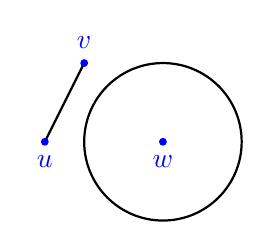
\begin{tikzpicture}
            % Define points
            \coordinate (u) at (1.5,0);
            \coordinate (v) at (2,1);
            \coordinate (w) at (3,0);

            % Draw the line segment from u to v
            \draw[thick] (u) -- (v);

            \draw[thick] (w) circle (1);

            % Label intersection points
            \node[circle,fill,color=blue,inner sep=1pt,label={[text=blue]-90:\(u\)}] at (u) [] {}; 
            \node[circle,fill,color=blue,inner sep=1pt,label={[text=blue, above]:\(v\)}] at (v) [] {}; 
            \node[circle,fill,color=blue,inner sep=1pt,label={[text=blue]-90:\(w\)}] at (w) [] {}; 
        \end{tikzpicture}
        \caption{\(\hat t_0, \hat t_1\) do not exist\\ \(\hat t_0' = \hat t_1' = \infty\)}
    \end{subfigure}
    \caption{The different kinds of solutions. Note that we associate \(0\) with \(u\), \(1\) with \(v\) and \(t\) with \((1-t)u + tv\)}
    \label{fig:solution_kinds}
\end{figure}

In general, determining these solutions requires finding roots of polynomials and thus there is no exact solution algorithm for Minkowski distances \(\delta_e\) for \(e > 4\) as such polynomials are not solvable. Here, we derive explicit solutions for the Euclidean Distance, the Manhattan Distance and the Chebyshev Distance. 

\subsubsection{Euclidean Distance}
\label{subsubsec:eq_euclidean_distance}
In the case of the Euclidean distance, \cref{eq:eq_solve_main} simplifies to the equation 
\begin{align*}
  \| (u - w) + t(v - u) \|_2 &= \varepsilon \\
  \| (u - w) + t(v - u) \|_2^2 &= \varepsilon^2 \\
  \| u - w \|_2^2 + 2\braket{u - w | v - u} t  +  \| v - u \|_2^2 t^2 &= \varepsilon^2 \\
  \underbrace{\delta(u,w)^2 - \varepsilon^2}_{\alpha_0} + \underbrace{2\braket{u - w | v - u} }_{\alpha_1}t  +  \underbrace{\delta(v, u)^2}_{\alpha_2} t^2 &= 0 \\
  \alpha_0 + \alpha_1 t  + \alpha_2 t^2 &= 0,
\end{align*}

which is a quadratic equation in \(t\) and can be solved explicitly as 

\begin{equation}
  t_{0,1} = \frac{-\alpha_1 \pm \sqrt{\alpha_1^2 - 4\alpha_0\alpha_2}}{2\alpha_2}.\label{eq:sol_explicit_euclidean}
\end{equation}

If the discriminant \(\alpha_1^2 - 4\alpha_0\alpha_2\) is smaller than \(0\) there is no solution. Otherwise we can compute the two solutions and have the lower and smallest and largest solution. 


\subsubsection{Manhattan Distance}
\label{subsubsec:eq_manhattan_distance}
In the case of the Manhattan distance, \cref{eq:eq_solve_main} simplifies to 
\begin{equation}
  \sum_{i=0}^d |u_i - w_i + t (v_i - u_i)| = \varepsilon. \label{eq:solve_manhattan}
\end{equation}

We note that \(|u_i - w_i + t (v_i - u_i )|\) can only assume the two values \(u_i - w_i + t(v_i - u_i)\) or \(w_i - u_i - t(v_i - u_i)\) depending on \(t\). For a fixed \(t\) we can evaluate all terms in the sum in \cref{eq:solve_manhattan} to get a linear equation in \(t\) which is trivial to solve, and the check if the resulting solution is valid. We define \(t_i \coloneq \frac{w_i - u_i}{v_i - u_i} \). Let \(\sigma:\set{1,\dots, d} \to \set{1,\dots, d}\) be the sorting permutation with \(t_{\sigma(1)} < t_{\sigma(2)} < \cdots < t_{\sigma(d)}\). For \(t \in [t_{\sigma(i)}, t_{\sigma(i+1)}]\) each of the terms in the sum can be simplified to a linear term without the absolute value and thus the whole sum degenerates into a linear equation which can be trivially solved. Finally we can check if the solution found for this interval does indeed lie in the interval. 

This whole process can be implemented na\"ively using a Sweepline algorithm in time \(\O(d^2)\) by constructing the values \(t_i\), sorting them and for each interval we compute the whole sum in linear time and solve the equation. As there are \(d\) many such values to consider we get quadratic runtime. We can improve this by using the fact that by iterating from smallest to largest during each testing step only a single term changes its sign, thus we can maintain the current linear equation and update it accordingly in constant time. The bulk of the computation now lies in sorting which gives us a runtime og \(\O(d \log d)\). 

There are a few edge cases, namely those being that multiple \(t_i\) coincide as well as that there are \(u_i = v_i\). The former case actually does not require special treatment as it will result in checking for a solution in an interval that contains only one value and at this value all with the same \(t_i\) will be zero. The second case degenerates the term into a constant which can be pulled out of the sum and into the right side.

\begin{algorithm}[ht]
  \DontPrintSemicolon
  \KwData{vectors \(u, v, w \in \R^d\), \(\varepsilon > 0\)}
  \KwResult{Solution to \cref{eq:solve_manhattan}}
  \BlankLine
  \(global\_slope \gets 0, global\_offset \gets 0\) \;
  \(events \gets Array(d)\)
  \For{\(i = 1, \dots, d\)}{
    \(slope \gets v_i - u_i, offset \gets u_i - w_i\)\;
    \If{\(slope < 0\)}{
      \(slope \gets -slope, offset \gets -offset\)
    } \ElseIf{\(slope = 0\)}{
      \(\varepsilon \gets \varepsilon - |offset|\)\;
      \Continue
    }
    \(zero \gets - \frac{offset}{slope}\)\;
    \If{\(zero \leq 0\)}{
      \(global\_offset \gets global\_offset + offset\)\;
      \(global\_slope \gets global\_slope + slope\)\;
      \Continue
    } 
    \(global\_offset \gets global\_offset - offset\)\;
    \(global\_slope \gets global\_slope - slope\)\;
    \If{\(zero \geq 1\)}{
      \Continue
    }
    \(events.append((zero, slope, offset))\)\;
  }
  Sort \(events\) by their \(zero\) component\;
  \(start \gets 0\)\;
  \For{\((zero, slope, offset) \in events\)}{
    Test if solution \(\frac{\varepsilon - global\_offset}{global\_slope} \in [start, zero]\) and report solution if so\;
    \(global\_offset \gets global\_offset + 2offset\)\;
    \(global\_slope \gets global\_slope + 2slope\)\;
    \(start \gets zero\)
  }
  Test if solution \(\frac{\varepsilon - global\_offset}{global\_slope} \in [start, 1]\) and report solution if so\;

  \caption{manhattan\_solver(\(u, v, w, \varepsilon\))}
  \label{algo:solve_manhattan}
\end{algorithm}


\subsubsection{Chebyshev Distance}
\label{subsubsec:eq_chebyshev_distance}
In the case of the Chebyshev distance \cref{eq:eq_solve_main} becomes 
\begin{equation}
  \max_{i = 1,\dots, d} |u_i - w_i + t(v_i - u_i)| = \varepsilon\label{eq:solve_chebyshev}
\end{equation}
for which a na\"ive solution can be found easily as the maximum will only assume as value one of the terms and each term has two possible values depending on the absolute value. Thus there are \(2d\) possible solutions which can be checked each in linear time if they indeed are the maximum resulting in a simple quadratic runtime algorithm. 

Just as in the case of the Manhattan distance, we only need to consider the solutions in the interval \([0,1]\) which eliminates possible solutions and in small dimensions this is probably the best choice. 

We can also reduce the runtime to \(d \log d\) by efficiently updating the current maximum. As each term is a line, we can find the initial maximum line at the start and update it when it crosses another line thus a modified version of the Bentley-Ottmann algorithm for line segment intersection (e.g. as explained in \cite{computational_geometry}) can be used where where the handling of intersections is modified to remove the line segment that falls below the other and only computing new intersections upwards. This guarantees that even if there are quadratically many intersecions only \(\O(d \log d)\) runtime is needed as irrelevant intersections are omitted. 
This allows a simplification in that we do not need a self-balancing binary search tree to store the line segments. A doubly linked list suffices as we remove for each intersection a line segment and the relative ordering remains the same. This list can be stored in an array where each array entry has an index to the previous and next line segment and its data, i.e., the offset and slope. A more detailed version of this idea can be seen in \cref{algo:solve_chebyshev} an example of the resulting line intersection problem can be seen in \cref{fig:chebyshev_algo}. For a full implementation, the case distinction in \cref{subsec:equation_solving} needs to be implemented, the handling of the marked solutions.

\begin{figure}
  \centering 
  \begin{subfigure}[h]{0.3\textwidth}
    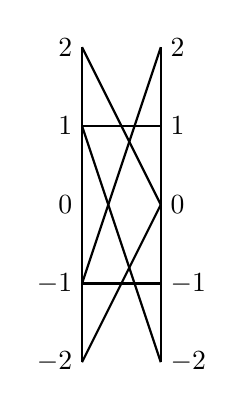
\begin{tikzpicture}
      % Draw the y-axes at x = 0 and x = 1
      \draw[thick] (0, -2) -- (0, 2) node[above] {};
      \draw[thick] (1, -2) -- (1, 2) node[above] {};

      % Add labels for the y-axis ticks
      \foreach \y in {-2, -1, 0, 1, 2} {
          \node[left] at (0, \y) {$\y$};
          \node[right] at (1, \y) {$\y$};
      }

      \draw[thick] (0,2) -- (1,0) node {};
      \draw[thick] (0,-2) -- (1,0) node {};
      \draw[thick] (0,1) -- (1,1) node {};
      \draw[thick] (0,-1) -- (1,-1) node {};
      \draw[thick] (0,-1) -- (1,2) node {};
      \draw[thick] (0,1) -- (1,-2) node {};
    \end{tikzpicture}
    \caption{All candidate lines}
  \end{subfigure}
  \begin{subfigure}[h]{0.3\textwidth}
    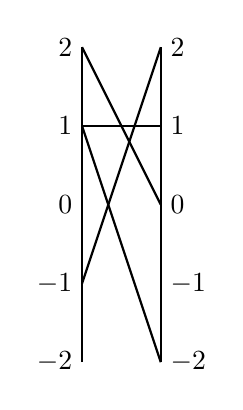
\begin{tikzpicture}
      % Draw the y-axes at x = 0 and x = 1
      \draw[thick] (0, -2) -- (0, 2) node[above] {};
      \draw[thick] (1, -2) -- (1, 2) node[above] {};

      % Add labels for the y-axis ticks
      \foreach \y in {-2, -1, 0, 1, 2} {
          \node[left] at (0, \y) {$\y$};
          \node[right] at (1, \y) {$\y$};
      }

      \draw[thick] (0,2) -- (1,0) node {};
      \draw[thick] (0,1) -- (1,1) node {};
      \draw[thick] (0,-1) -- (1,2) node {};
      \draw[thick] (0,1) -- (1,-2) node {};
    \end{tikzpicture}
    \caption{Lines that are not fully negative}
  \end{subfigure}
  \begin{subfigure}[h]{0.3\textwidth}
    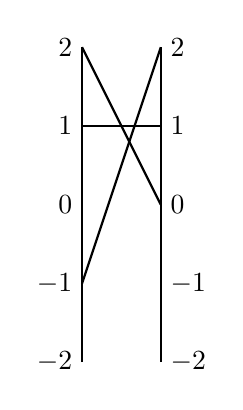
\begin{tikzpicture}
      % Draw the y-axes at x = 0 and x = 1
      \draw[thick] (0, -2) -- (0, 2) node[above] {};
      \draw[thick] (1, -2) -- (1, 2) node[above] {};

      % Add labels for the y-axis ticks
      \foreach \y in {-2, -1, 0, 1, 2} {
          \node[left] at (0, \y) {$\y$};
          \node[right] at (1, \y) {$\y$};
      }

      \draw[thick] (0,2) -- (1,0) node {};
      \draw[thick] (0,1) -- (1,1) node {};
      \draw[thick] (0,-1) -- (1,2) node {};
    \end{tikzpicture}
    \caption{Lines that are not fully below another line}
  \end{subfigure}\\
  \begin{subfigure}[h]{0.3\textwidth}
    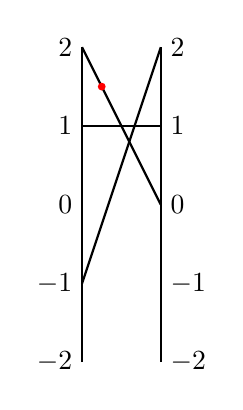
\begin{tikzpicture}
      % Draw the y-axes at x = 0 and x = 1
      \draw[thick] (0, -2) -- (0, 2) node[above] {};
      \draw[thick] (1, -2) -- (1, 2) node[above] {};

      % Add labels for the y-axis ticks
      \foreach \y in {-2, -1, 0, 1, 2} {
          \node[left] at (0, \y) {$\y$};
          \node[right] at (1, \y) {$\y$};
      }

      \draw[thick] (0,2) -- (1,0) node {};
      \draw[thick] (0,1) -- (1,1) node {};
      \draw[thick] (0,-1) -- (1,2) node {};

      \node[circle,fill,color=red,inner sep=1pt] at (0.25, 1.5) {};
    \end{tikzpicture}
    \caption{Find next intersection. Here between topmost line so check for solution.}
  \end{subfigure}
  \begin{subfigure}[h]{0.3\textwidth}
    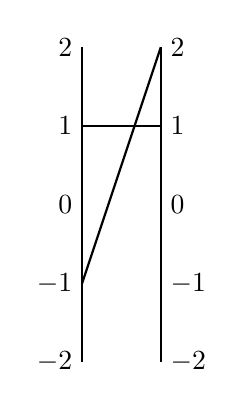
\begin{tikzpicture}
      % Draw the y-axes at x = 0 and x = 1
      \draw[thick] (0, -2) -- (0, 2) node[above] {};
      \draw[thick] (1, -2) -- (1, 2) node[above] {};

      % Add labels for the y-axis ticks
      \foreach \y in {-2, -1, 0, 1, 2} {
          \node[left] at (0, \y) {$\y$};
          \node[right] at (1, \y) {$\y$};
      }

      \draw[thick] (0,1) -- (1,1) node {};
      \draw[thick] (0,-1) -- (1,2) node {};

    \end{tikzpicture}
    \caption{Find next intersection. No solution found}
  \end{subfigure}
  \begin{subfigure}[h]{0.3\textwidth}
    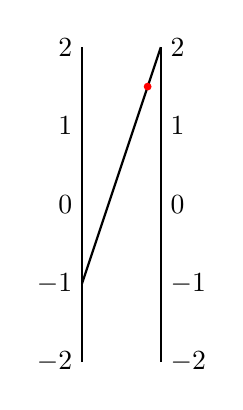
\begin{tikzpicture}
      % Draw the y-axes at x = 0 and x = 1
      \draw[thick] (0, -2) -- (0, 2) node[above] {};
      \draw[thick] (1, -2) -- (1, 2) node[above] {};

      % Add labels for the y-axis ticks
      \foreach \y in {-2, -1, 0, 1, 2} {
          \node[left] at (0, \y) {$\y$};
          \node[right] at (1, \y) {$\y$};
      }

      \draw[thick] (0,-1) -- (1,2) node {};
      \node[circle,fill,color=red,inner sep=1pt] at (0.833, 1.5) {};
    \end{tikzpicture}
    \caption{Check final line for an intersection}
  \end{subfigure}


  \caption{Line representation of the equation \(\delta_\infty((0,0,0) + t(-2,0,3), (-2,-1,1)) = 1.5\)}
  \label{fig:chebyshev_algo}
\end{figure}

\begin{algorithm}[ht]
  \DontPrintSemicolon
  \KwData{vectors \(u, v, w \in \R^d\), \(\varepsilon > 0\)}
  \BlankLine
  \(candidates \gets \set{(2i, u_i - w_i, v_i - u_i), (2i+1, w_i - u_i, u_i - v_i) | i = 0, \dots, d - 1}\) \;
  \(queue \gets PriorityQueue()\) \;
  \(list \gets Array(|candidates|)\) \;
  sort candidates according to second component descendingly,
  in case of ties use the third component as tie breaker descendingly \;
  \(PREV \gets 0, NEXT \gets 1\) \tcp{constants for readability}
  \(curr \gets -1\) \;
  \For{\((i, a, b) \in candidates\)}{
    \If{\(curr = -1\)} {
      \(curr \gets i, a' \gets a, b' \gets b\)\;
      \(list[curr] \gets (-1, -1, a, b)\) \;
      \Continue
    } 

    \If{\( a' + b' \geq a + b\)}{
      \Continue \tcp{new line fully below current line so never maximum}
    } 

    \(list[curr][NEXT] \gets i, list[i] \gets (curr, -1, a, b)\) \;
    \(intersection \gets \frac{a' - a}{b - b'}\) \tcp{always in \([0,1]\)}
    \(queue.insert\_with\_priority((curr, i), intersection)\) \;
    \(curr \gets i, a' \gets a, b' \gets b\) \;
  }

  \caption{chebyshev\_solver\_initialization(\(u, v, w\))}
  \label{algo:solve_chebyshev_init}
\end{algorithm}

\begin{algorithm}[ht]
  \DontPrintSemicolon
  \KwData{vectors \(u, v, w \in \R^d\), \(\varepsilon > 0\)}
  \KwResult{Solution to \cref{eq:solve_chebyshev}}
  \BlankLine
  \(chebyshev\_solver\_initialization(u, v, w)\) \;
  \(last\_intersection \gets 0\) \;
  \While{\(\lnot queue.empty()\)}{
    \((i, j), intersection \gets queue.poll()\) \;
    \If{\(list[i][PREV] = -1 \lor list[j][PREV] = -1\)}{
      \Continue \tcp{One of the lines already removed, no intersection}
    } 
    \If{\(i = HEAD\)}{
      \(HEAD \gets j\) \;
      \(\_, \_, a, b \gets list[i]\) \;
      \If{\(b = 0\)}{
        \If{\(a = \varepsilon\) }{
          Mark \(last\_intersection\) as earliest solution or \(intersection\) as last solution \;
        }
        \(last\_intersection \gets intersection\) \;
        \Continue 
      }
      \(solution \gets \frac{\varepsilon - a}{b}\) \;
      Mark \(solution\) as earliest or last solution if \(solution \in [last\_intersection, intersection]\) \;
      \(last\_intersection \gets intersection\) \;
      \Continue
    }
    \(before_i \gets list[i][PREV]\) \;
    \(list[before_i][NEXT] \gets j, list[j][PREV] \gets before_i\) \;
    \(list[i][PREV] \gets -1\) \tcp{mark as removed}
    \(last\_intersection \gets intersection\) \;
    \If{\(before_i \neq HEAD\)}{
      \(\_, \_, a, b \gets list[j]\) \;
      \(\_, \_, a', b' \gets list[before_i]\) \;
      \(intersection \gets \frac{a' - a}{b - b'}\) \tcp{also in \([0,1]\)}
      \(queue.insert\_with\_priority((before_i, j), intersection)\) \;
    }
  }
  Check for solution in \([last\_intersection, 1]\) \;

  \caption{chebyshev\_solver(\(u, v, w, \varepsilon\))}
  \label{algo:solve_chebyshev}
  
\end{algorithm}

\subsection{\(\O(k^*n^5)\) Algorithm}
\label{subsec:simple_algo}

In this subsection we will sketch \citeauthor{on_optimal_polyline_simplification_using_the_hausdorff_and_frechet_distance}'s algorithm for polyline simplification as well as a simplified version of \citeauthor{computing_the_frechet_distance_between_two_polygonal_curves}'s algorithm to decide if two polylines have Fréchet distance of at most \(\varepsilon\). 

\subsubsection{Fréchet Distance Decision Algorithm}
\label{ssec:alt_godau}
The simplification algorithm we will describe heavily uses a subroutine to solve the following problem: Given \(\varepsilon > 0\), a polyline \(P \) of length \(p\), a polyline segment \(P[j' + t' \dots j+1]\) and a line segment \(\overline{P(i')P(i)}\) for \(i' < i \leq p, j' \leq j < p\in \N\) and \(t \in [0, 1]\). Decide if there is a \(t' \in [0, 1]\) such that \(\delta^F(P[j' + t' \dots j + t], \overline{P(i')P(i)}) \leq \varepsilon\) and if so determine the smallest such \(t\).  

This can be solved by a simplified version of \citeauthor{computing_the_frechet_distance_between_two_polygonal_curves}'s algorithm to decide if the Fréchet distance of two polylines is at most \(\varepsilon\). We present the algorithm in the specific form needed for this problem. 

In both cases we require that \(\delta(P(j' + t'), P(i')) \leq \varepsilon\) as the starting points of both polylines must match by definition. If this is not the case we can return that there is no such \(t\). We set \(t_0 \coloneq \hat t_0'(\overline{P(j)P(j+1)}, P(i))\) and \(t_1 \coloneq \hat t_1'(\overline{P(j)P(j+1)}, P(i))\). As the end points must match, we get that \(t \in [t_0, t_1]\). Thus if there are no such interval we can also return that there is no solution.

We distinguish the two cases \(j' = j\) and \(j' < j\). 
\begin{enumerate}
  \item[\(j' = j\): ] In this case both \(t'\) and \(t\) lie on the same line segment \(\overline{P(j)P(j+1)}\) (which is the only line segment of the polyline segment). The only constraints on \(t\) are that \(t \in [t', 1]\) and \(t \in [ t_0, t_1]\) which is possible if and only if \(t' \leq t_1\). If this is the case the solution is \(\max(t', t_0)\).

  \item[\(j' < j\): ] In this case we iterate over all points of the polyline segment \(P(k) = P(j'+1), \dots, P(j)\) and compute the solutions \(\hat t_0'(\overline{P(i')P(i)}, P(k)), \hat t_0'(\overline{P(i')P(i)}, P(k))\). We maintain the first reachable point \(t'\) (initially \(0\)) on the line segment \(\overline{P(i')P(i)}\) for these points and test if \(t' \leq \hat t_0'(\overline{P(i')P(i)}, P(k))\). If that is the case we can update it \(t' \gets \max(t', \hat t_0'(\overline{P(i')P(i)}, P(k)))\). If this is not possible at any step we can return that there is no solution. Otherwise, we have fully traversed the line segment and most of the polyline segment. At this point the solution is merely \(t_0\).
\end{enumerate}

\subsubsection{Polyline Simplification Algorithm}
\label{ssec:simple_algo_main}

Here we outline the global polyline simplification algorithm from \citeauthor{on_optimal_polyline_simplification_using_the_hausdorff_and_frechet_distance} which we have implemented and tested for the Euclidean distance, the Manhattan distance, and the Chebyshev distance. 

Similar to the decision problem we use a dynamic program in which we store the earliest reachable points although in a more complicated manner. We construct a three dimensional table \(DP\) with entries in \([0, 1] \cup \set{\infty}\) for each triple \((k, i, j)\) with \(k, i \in \set{0, \dots, n}\) and \(j \in \set{0, \dots, n - 1}\) where \(n\) is the length of the given polyline \(P\). 

Each entry \(DP[k, i, j]\) stores the smallest \(t \in [0, 1]\) s.t. there is a simplification \(Q\) of \(P[0 \dots i]\) with exactly \(k\) line segments with \(\delta^F(Q, P[0\dots j + t]) \leq \varepsilon\). If no such \(t\) exists we store \(\infty\) in that entry. 
The solution is the smallest \(k^*\) s.t. \(DP[k^*, n, n - 1]\) exists, i.e., there is a simplification \(Q\) of the whole polyline with \(k^*\) many line segments that has \(\delta^F(Q, P[0\dots n - 1 + t]) \leq \varepsilon\) for some \(t \in [0, 1]\) so we can complete the simplification by simply going from \(n-1+t\) to \(n\) on the last line segment of \(P\) while staying on the last point of the simplification. 

For \(k = 0\) it is trivial to compute the entries. If \(i > 0\) we can store \(\infty\) as it is impossible to create a simplification of size \(0\) that goes to any point other than the first point. To find \(DP[0, 0, j]\) we only need to compute the distances from \(P(0)\) to the points \(P(j)\) (see \cref{fig:simpl_init}). Until the first \(j\) with \(\delta(P(0), P(j)) > \varepsilon\) we can store \(0\). From the first such \(j\) we store \(\infty\). This is because the simplification only consists of a single point \(P(0)\) thus the condition \(\delta^F(Q, P[0\dots j + t]) \leq \varepsilon\) simplifies to \(\delta^F(P[0 \dots 0], P[0 \dots j + t])\) and as we cannot move on the single point \(P(0)\) the earliest reachable point on each line segment must be \(t = 0\). 

The correctness of this initialization can be shown rather easily. 
\begin{lemma}
  Let \(P = \angl{P(0)}\) a polyline consisting of a single point and \(Q\) be a polyline of size \(n\). Then \(\delta^F(P, Q) \leq \varepsilon\) if, and only if, \(\delta(P(0), Q(i)) \leq \varepsilon\) for all \(i \in \set{0, \dots, n}\). 
\end{lemma}
\begin{proof}
  For \(\Rightarrow\) we must have some function \(f\) with \(\delta(Q(t), P(f(t))) \leq \varepsilon\) for all \(t\in [0,n]\) where \(f(0 ) = 0\) and \(f(n) = 0\) and \(f\) is  monotone, meaning that \(\delta(P(0), Q(t)) \leq \varepsilon\) and thus especially for \(t\in \set{0, \dots, n}\).
  
  For \(\Leftarrow\) we show that every point on \(Q\) has distance at most \(\varepsilon\) from \(P(0)\) thus we can choose any suitable function \(f\). This follows directly from property 3 from \cref{lem:distance_properties} applied to all individual line segment on \(Q\).
\end{proof}

\begin{figure}[b]
    \centering
    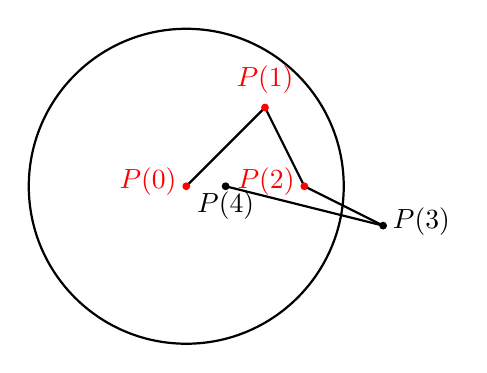
\begin{tikzpicture}[scale=0.5]
        % Define points
        \coordinate (p0) at (0, 0);

        \coordinate (p1) at (2, 2);
        \coordinate (p2) at (3, 0);

        \coordinate (p3) at (5, -1);
        \coordinate (p4) at (1, 0);

        \draw[thick] (p0) -- (p1);
        \draw[thick] (p1) -- (p2);
        \draw[thick] (p2) -- (p3);
        \draw[thick] (p3) -- (p4);

        \draw[thick] (p0) circle (4);

        \node[circle,fill,color=red,inner sep=1pt,label={[text=red, left]:\(P(0)\)}] at (p0) [] {}; 
        \node[circle,fill,color=red,inner sep=1pt,label={[text=red, above]:\(P(1)\)}] at (p1) [] {}; 
        \node[circle,fill,color=red,inner sep=1pt,label={[text=red, left]:\(P(2)\)}] at (p2) [] {}; 
        \node[circle,fill,color=black,inner sep=1pt,label={[text=black, right]:\(P(3)\)}] at (p3) [] {}; 
        \node[circle,fill,color=black,inner sep=1pt,label={[text=black, below]:\(P(4)\)}] at (p4) [] {}; 

    \end{tikzpicture}
  \caption{Initialization of the simplification algorithm for \(k = 0, i = 0\). Only the points in the circle until \(P(2)\) are reachable.}
  \label{fig:simpl_init}
\end{figure}


As for the other entries, the authors show that the entry \(DP[k, i, j]\) can be computed by the minimization over all \(i' < i\) and \(j' \leq j\). We lookup the value \(t \coloneq DP[k-1, i', j']\) and test if there is a \(t' \in [0, 1]\) s.t. \(\delta^F(P[j' + t' \dots j + t], \overline{P(i')P(i)}) \leq \varepsilon\) and return the smallest such \(t\) if possible. This can be done with the algorithm from \citeauthor{computing_the_frechet_distance_between_two_polygonal_curves} with the mentioned modifications. Among all those candidates \(t\) we choose the minimal one. If no such \(t\) exists we can store \(\infty\).

\begin{algorithm}[ht]
  \DontPrintSemicolon
  \KwData{Polyline \(P\) of length \(n\), \(\varepsilon > 0\)}
  \KwResult{Smallest \(\varepsilon\)-simplification of \(P\)}
  \BlankLine
  \(DP \gets Array((n + 1, n + 1, n))\) initialized with \(\infty\) \;
  \For{\(j = 0, \dots, n\)}{
    \If{\(\delta(P(0), P(j)) > \varepsilon\)}{
      \Break
    }
    \(DP[0, 0, j] \gets 0\)
  }
  \For{\(k=1,\dots\) until \(DP[k, n, n-1] \neq \infty\)}{
    \For{\(i=0,\dots, n\)}{
      \For{\(j=0,\dots, n-1\)}{
        \For{\(i' < i\)}{
          \For{\(j' \leq j\)}{
            Let \(t' \gets DP[k-1, i', j']\)\;
            Let \(t \gets AltGodau(P[j' + t' \dots j + 1], \overline{P(i')P(i)}, \varepsilon)\)\;
            \(DP[k, i, j] \gets min(DP[k, i, j], t)\)
          }
        }
      }
    }
  }
  \caption{PolylineSimplification(\(P, \varepsilon\))}
  \label{algo:simplify_simple}
\end{algorithm}

There are \(\O(k^* n^2)\) many iterations to fill in the table and each entry requires \(\O(n^2)\) many computations to find the minimum. Each call to the \(AltGodau\) subroutine requires linear runtime thus in total we have \(\O(k^*n^5)\) run time.

\subsection{Examples}
Before going into possible optimizations, we want to go through an example for the algorithm as well as the \citeauthor{computing_the_frechet_distance_between_two_polygonal_curves} subroutine. This gives us more intuition for the algorithms as well as ideas for further optimizations. Because of cubic amount of entries it is unreasonable to show all computations thus we only show the computations that lead to the simplification and the subroutine for them. 

\begin{figure}
  \centering
  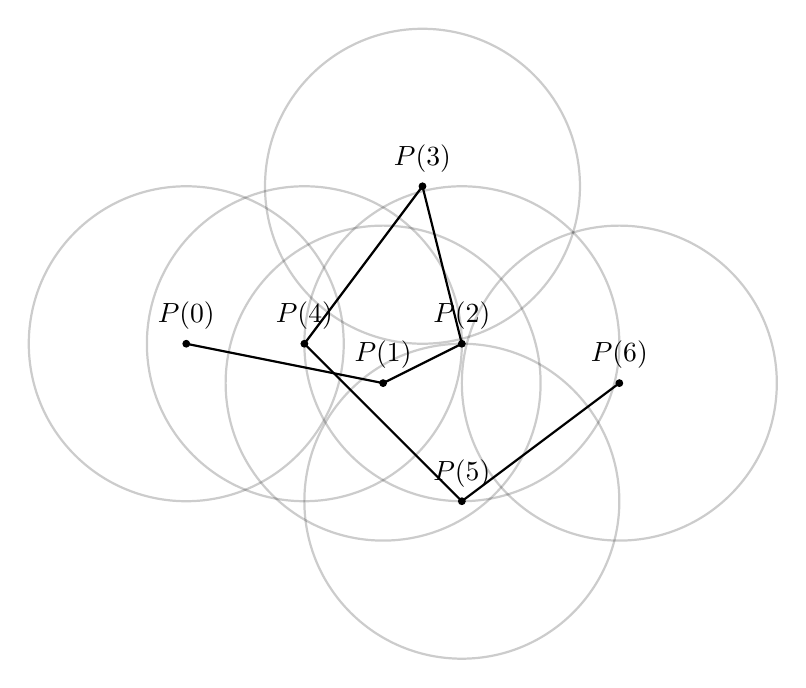
\begin{tikzpicture}[scale=0.5]
    \foreach \i/\x/\y in {0/0/0, 1/5/-1, 2/7/0, 3/6/4, 4/3/0, 5/7/-4, 6/11/-1}{
      \coordinate (p\i) at (\x, \y);
      \node[circle,fill,color=black,inner sep=1pt,label={[text=black, above]:\(P(\i)\)}] at (p\i) [] {}; 
      \draw[thick, opacity=0.2] (p\i) circle (4);
    }
    \foreach \i in {0,...,5}{
      \pgfmathsetmacro{\next}{\i+1}
      \draw[thick] (p\i) -- (p\next);
    }
  \end{tikzpicture}
  \caption{Example polyline with circles with radius \(\varepsilon\) drawn around all points. We note the following relations which may be hard to notice: \(\delta(P(2), P(4)) = \delta(P(2), P(5)) = \varepsilon\), \(\delta(P(2), P(3)) > \varepsilon\), \(\delta(P(2), P(6)) > \varepsilon\).}
  \label{fig:poly-ex-main}
\end{figure}

For the polyline and \(\varepsilon\) in \cref{fig:poly-ex-main} we initialize the table layer for \(k = 0\) by only setting the value \(DP[0,0,0]\) to \(0\) as \(\delta(P(0), P(1)) > \varepsilon\). Even though \(\delta(P(0), P(4)) \leq \varepsilon\) the value \(DP[0,0,4]\) is \(\infty\) as there are points between that already fail.

For the layer \(k = 1\) we can only procede from the entry \(DP[0,0,0] = 0\) as it is the only one we found on the previous layer. All triples \(k, i, j\) for which a valid entry in \([0, 1]\) can be found for the layer \(k = 1\) are listed in \cref{tab:exlayer1}. The respective \(i', j'\) and \(t'\) are not listed as there is only one possible entry.
\begin{table}[h]
\centering
\begin{tabular}{|ccc|}
\hline
$(1,1,0)$ & $(1,1,1)$ & $(1,1,2)$ \\
$(1,2,0)$ & $(1,2,1)$ & $(1,2,2)$ \\
$(1,2,3)$ & $(1,2,4)$ & $(1,2,5)$ \\
$(1,3,2)$ & $(1,3,3)$ & $(1,4,0)$ \\
$(1,4,1)$ & $(1,4,2)$ & $(1,5,0)$ \\
$(1,5,1)$ & $(1,5,2)$ & \\
\hline
\end{tabular}
\caption{Valid entries for layer \(k = 1\). All procede from \((0,0,0)\).}
\label{tab:exlayer1}
\end{table}

Let us explicitly go through the AltGodau subroutine for the entry \((1, 2, 3)\). i.e., A simplification consisting of one line segment for the polyline \(P[0\dots 2]\) that has distance of at most \(\varepsilon\) to \(P[j' + t'\dots j + t] = P[0 \dots 3 + t]\) where \(t\) is gotten from the subroutine. We consider the line segment \(\overline{P(i')P(i)} = \overline{P(0)P(2)}\) and the polyline segment \(P[j' + t' \dots j + 1] = P[0 \dots 4]\) and perform the algorithm. 

\begin{figure}
  \centering
  \begin{subfigure}[b]{0.4\textwidth}
    \begin{tikzpicture}[scale=0.4]
      \foreach \i/\x/\y in {0/0/0, 1/5/-1, 2/7/0, 3/6/4, 4/3/0, 5/7/-4, 6/11/-1}{
        \coordinate (p\i) at (\x, \y);
        \node[circle,fill,color=black,inner sep=1pt,label={[text=black, above]:\(P(\i)\)}] at (p\i) [] {}; 
      }
      \foreach \i in {0,...,5}{
        \pgfmathsetmacro{\next}{\i+1}
        \draw[thick] (p\i) -- (p\next);
      }

      \path[name path=line] (p0) -- (p2);
      \path[name path=circle] (p1) circle (4);
      \path[name intersections={of=line and circle, by={t0,t1}}];

      \draw[thick, opacity=0.2] (p1) circle (4);
      \draw[color=red, dotted, thick] (p0) -- (p2);
      \draw[color=blue, thick] (p0) -- (p1);
      \draw[color=blue, thick] (p0) -- (t0);
    \end{tikzpicture}
  \end{subfigure}
  \begin{subfigure}[b]{0.4\textwidth}
    \begin{tikzpicture}[scale=0.4]
      \foreach \i/\x/\y in {0/0/0, 1/5/-1, 2/7/0, 3/6/4, 4/3/0, 5/7/-4, 6/11/-1}{
        \coordinate (p\i) at (\x, \y);
        \node[circle,fill,color=black,inner sep=1pt,label={[text=black, above]:\(P(\i)\)}] at (p\i) [] {}; 
      }
      \foreach \i in {0,...,5}{
        \pgfmathsetmacro{\next}{\i+1}
        \draw[thick] (p\i) -- (p\next);
      }

      \path[name path=line] (p0) -- (p2);
      \path[name path=circle1] (p1) circle (4);
      \path[name intersections={of=line and circle1, by={t00,t10}}];
      \path[name path=circle2] (p2) circle (4);
      \path[name intersections={of=line and circle2, by={t01,t11}}];

      \draw[thick, opacity=0.2] (p2) circle (4);
      \draw[color=red, dotted, thick] (p0) -- (p2);
      \draw[color=blue, thick] (p1) -- (p2);
      \draw[color=blue, thick] (t00) -- (t01);
    \end{tikzpicture}
  \end{subfigure}\\
  \begin{subfigure}[b]{0.4\textwidth}
    \begin{tikzpicture}[scale=0.4]
      \foreach \i/\x/\y in {0/0/0, 1/5/-1, 2/7/0, 3/6/4, 4/3/0, 5/7/-4, 6/11/-1}{
        \coordinate (p\i) at (\x, \y);
        \node[circle,fill,color=black,inner sep=1pt,label={[text=black, above]:\(P(\i)\)}] at (p\i) [] {}; 
      }
      \foreach \i in {0,...,5}{
        \pgfmathsetmacro{\next}{\i+1}
        \draw[thick] (p\i) -- (p\next);
      }
      \path[name path=line] (p0) -- (p2);
      \path[name path=circle1] (p2) circle (4);
      \path[name intersections={of=line and circle1, by={t00,t10}}];
      \path[name path=circle2] (p3) circle (4);
      \coordinate (t01) at (6,0);

      \draw[thick, opacity=0.2] (p3) circle (4);
      \draw[color=red, dotted, thick] (p0) -- (p2);
      \draw[color=blue, thick] (p2) -- (p3);
      \draw[color=blue, thick] (t00) -- (t01);
    \end{tikzpicture}
  \end{subfigure}
  \begin{subfigure}[b]{0.4\textwidth}
    \begin{tikzpicture}[scale=0.4]
      \foreach \i/\x/\y in {0/0/0, 1/5/-1, 2/7/0, 3/6/4, 4/3/0, 5/7/-4, 6/11/-1}{
        \coordinate (p\i) at (\x, \y);
        \node[circle,fill,color=black,inner sep=1pt,label={[text=black, above]:\(P(\i)\)}] at (p\i) [] {}; 
      }
      \foreach \i in {0,...,5}{
        \pgfmathsetmacro{\next}{\i+1}
        \draw[thick] (p\i) -- (p\next);
      }
      % same point
      \coordinate (t00) at (6,0);
      \path[name path=line] (p3) -- (p4);
      \path[name path=circle] (p2) circle (4);
      \path[name intersections={of=line and circle, by={t0,t1}}];

      \draw[thick, opacity=0.2] (p2) circle (4);
      \draw[color=red, dotted, thick] (p0) -- (p2);
      \draw[color=red, thick] (p3) -- (t0);
      \draw[color=blue, thick] (t00) -- (p2);
    \end{tikzpicture}
  \end{subfigure}
  \caption{Finding the first reachable point on \(\overline{P(3)P(4)}\). Resulting in \(t = 0.04\) marginally below point \(P(3)\). Note again that \(\delta(P(2), P(3)) > \varepsilon\). The point \(P(4)\) is not part of the simplification, it only lies on the line segment \(\overline{P(0)P(2)}\) by chance.}
  \label{fig:poly-ex-123-ag}
\end{figure}

From \(DP[1,2,3] = 0.04\) we can procede to the end of the polyline to get a simplification of size \(2\) as seen in \cref{fig:poly-ex-265-ag}. A simplification of size \(1\) is not possible as that would be the line segment \(\overline{P(0)P(6)}\) but there is no point on that line segment that has distance \(\leq \varepsilon\) from \(P(3)\). 

\begin{figure}
  \centering
  \begin{subfigure}[b]{0.4\textwidth}
    \begin{tikzpicture}[scale=0.4]
      \foreach \i/\x/\y in {0/0/0, 1/5/-1, 2/7/0, 3/6/4, 4/3/0, 5/7/-4, 6/11/-1}{
        \coordinate (p\i) at (\x, \y);
        \node[circle,fill,color=black,inner sep=1pt,label={[text=black, above]:\(P(\i)\)}] at (p\i) [] {}; 
      }
      \foreach \i in {0,...,5}{
        \pgfmathsetmacro{\next}{\i+1}
        \draw[thick] (p\i) -- (p\next);
      }

      \path[name path=line] (p3) -- (p4);
      \path[name path=circle] (p2) circle (4);
      \path[name intersections={of=line and circle, by={t0,t1}}];

      \draw[thick, opacity=0.2] (p4) circle (4);
      \draw[color=red, dotted, thick] (p2) -- (p6);
      \node[circle,fill,color=blue,inner sep=1pt] at (p2) [] {}; 
      \draw[color=blue, thick] (t0) -- (p4);
    \end{tikzpicture}
  \end{subfigure}
  \begin{subfigure}[b]{0.4\textwidth}
    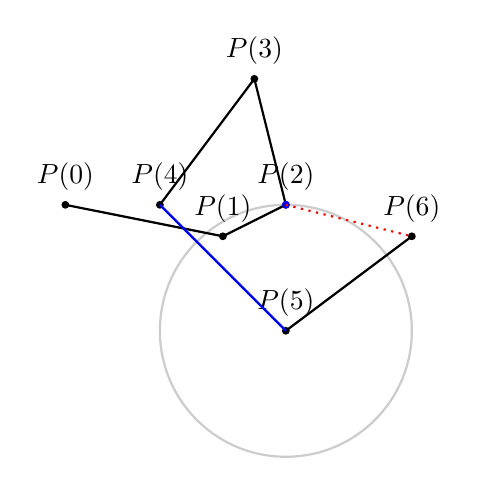
\begin{tikzpicture}[scale=0.4]
      \foreach \i/\x/\y in {0/0/0, 1/5/-1, 2/7/0, 3/6/4, 4/3/0, 5/7/-4, 6/11/-1}{
        \coordinate (p\i) at (\x, \y);
        \node[circle,fill,color=black,inner sep=1pt,label={[text=black, above]:\(P(\i)\)}] at (p\i) [] {}; 
      }
      \foreach \i in {0,...,5}{
        \pgfmathsetmacro{\next}{\i+1}
        \draw[thick] (p\i) -- (p\next);
      }

      \node[circle,fill,color=blue,inner sep=1pt] at (p2) [] {}; 
      \draw[thick, opacity=0.2] (p5) circle (4);
      \draw[color=red, dotted, thick] (p2) -- (p6);
      \draw[color=blue, thick] (p4) -- (p5);
    \end{tikzpicture}
  \end{subfigure}\\
  \begin{subfigure}[b]{0.4\textwidth}
    \begin{tikzpicture}[scale=0.4]
      \foreach \i/\x/\y in {0/0/0, 1/5/-1, 2/7/0, 3/6/4, 4/3/0, 5/7/-4, 6/11/-1}{
        \coordinate (p\i) at (\x, \y);
        \node[circle,fill,color=black,inner sep=1pt,label={[text=black, above]:\(P(\i)\)}] at (p\i) [] {}; 
      }
      \foreach \i in {0,...,5}{
        \pgfmathsetmacro{\next}{\i+1}
        \draw[thick] (p\i) -- (p\next);
      }
      \path[name path=line] (p5) -- (p6);
      \path[name path=circle] (p6) circle (4);
      \path[name intersections={of=line and circle, by={t0,t1}}];

      \draw[thick, opacity=0.2] (p6) circle (4);
      \draw[color=blue, thick] (p2) -- (p6);
      \draw[color=blue, thick] (p5) -- (t0);
    \end{tikzpicture}
  \end{subfigure}
  \caption{Finding the first reachable point on \(\overline{P(5)P(6)}\). With that we have found a simplification for the whole polyline.}
  \label{fig:poly-ex-265-ag}
\end{figure}


For completeness sake the entries on the layer \(k = 2\) are listed in \cref{tab:exlayer2}. The entry \((k - 1, i', j')\) they reference from the previous layer is added after the tuple. This predecessor tuple is not necessarily unique, in fact, every single one of these has at least two different possibilities for \(i', j'\).
\begin{table}[h]
\centering
\begin{tabular}{|ccc|}
\hline
$(2,4,3):(2, 1)$ & $(2,4,4):(2, 1)$ & $(2,5,4):(2,4)$ \\
$(2,5,5):(2,4)$ & $(2,6,5):(2,4)$ & \\
\hline
\end{tabular}
\caption{Valid entries for layer \(k = 1\). All procede from \((0,0,0)\).}
\label{tab:exlayer2}
\end{table}

\subsection{Optimizations}
\label{ssec:optimizations}
Based on the just described algorithm we outline optimizations that greatly reduce the \(\O(k^*n^5)\) runtime in practice or improve upon the algorithm in terms of space and numerical stability. The most effective optimizations circumvent the theoretical runtime by skipping iterations. 

We first note that for the entry \((k, i, j)\) in the dynamic program we do not always need to iterate over all possible \(i' < i\) and \(j' \leq j\). As we are interested in the minimal value \(t\) on the line segment \(\overline{v_{j}v_{j+1}}\) that can be reached, we can stop further search if we have reached a lower bound for that value. Such a lower bound is \(\hat t_0'(\overline{v_{j}v_{j+1}}, i)\), i.e. the modified solution to the \cref{eq:eq_solve_main}, which is tight as for a sufficiently large \(k\) this value must be reached eventually. This allows an early break out of the search through the \(i' < i, j'\leq j\) and a speed up of upto quadratic runtime. 

Another optimization based on a similar insight is the following: If the entry at \((k-1, i, j) = \hat t_0'(\overline{v_{j}v_{j+1}}, i)\), i.e., we have found a simplification for the same \(i\) and \(j\) that has already reached the optimal value, we know this cannot be improved in the current layer \(k\) or any further one. This means, the entry at \((k, i, j)\) can never be used by some entry \((k + 1, i'', j'')\) because of minimality as any such entry that uses \((k, i, j)\) could have already used \((k-1, i, j)\) for \((k, i'', j'')\). This allows us to completely ignore the computation of the value. This allows a continuous speed up of the algorithm while it runs as once this happens for an entry, it will happen for all further ones with a higher value of \(k\) so with each layer more entry computations can be skipped. 

Another way to skip computations is to ignore all \(i\) with \(i < k\) as well as all \(i'\) with \(i' < k - 1\) in the computations as there can never be a simplification of \(P[0\dots i]\) that uses more than \(i\) line segments thus it must always hold that \(i \geq k\). 

A last simple optimization of a similar type which is particularly useful for well-behaved polylines is to not even start the iterations over the \(i', j'\) if there is no solution \(\hat t_0'(\overline{v_{j}v_{j+1}}, i)\). This happens often if there are not too many line segments close to each other.











%\subsection{Cubic Runtime Algorithm}
%\label{subsec:refined_algo}

\subsection{Implementation}
\label{subsec:implementation}
% details 
% decision problem: is which intersection point comes first instead of explicit computation 
%   does not need sqrt for euclidean distance, no roots for general norms, allows binary search to estimate intervals 
%   only using the distance function instead of root solving algorithm 
%
% only use min(p, q) space instead of p * q space for decision variant (especially for our case constant extra space)
%




\section{Implicit Polyline Simplification}\label{sec:implicit_polyline_simplification}
In this section, we review the polyline simplification algorithm and all of its dependencies in order to avoid explicitly computing the solutions of distance equations. We abstract the instances in \citeauthor{on_optimal_polyline_simplification_using_the_hausdorff_and_frechet_distance}'s algorithm for polyline simplification and the required Fréchet distance decision algorithm from \citeauthor{computing_the_frechet_distance_between_two_polygonal_curves} that require explicit solutions to these equations, reducing them to a small set of decision problems.
We show how these decision problems can be solved for the Euclidean distance without using square roots or even divisions, meaning only addition, subtraction, and multiplication are required. The correctness of the implicit algorithms follows directly from the correctness of the explicit version, as only the method of comparison is abstracted while the underlying logic remains unaffected.

\subsection{Related Works}
To our knowledge, all existing algorithms that make use of the Fréchet distance employ the real RAM \cite{computational_geometry_shamos} as their computational model. This model enables storing real numbers and operating on them with addition, subtraction, multiplication, and division in constant time. Furthermore, for the Euclidean distance, it is assumed that square roots can be computed in constant time, and when extending results to arbitrary distance functions, it is assumed that the necessary equations can be solved. \citeauthor{computing_the_frechet_distance_between_two_polygonal_curves}~\cite{computing_the_frechet_distance_between_two_polygonal_curves}, \citeauthor{on_optimal_polyline_simplification_using_the_hausdorff_and_frechet_distance}~\cite{on_optimal_polyline_simplification_using_the_hausdorff_and_frechet_distance}, and \citeauthor{polyline_simplification_has_cubic_complexity_bringmannetal}~\cite{polyline_simplification_has_cubic_complexity_bringmannetal} all present their algorithms in this model, as do many others.

We review the structure of these equation solutions and observe that arbitrary real numbers are not strictly necessary. The implicit approach requires the least powerful computational model in theory by abstracting the equation solving away into the necessary comparisons. Using suitable representations for the involved numbers allows us to assume the regular RAM, at least for the Euclidean, Manhattan, and Chebyshev distances. Whether this suffices for arbitrary Minkowski distances remains an open problem.

\subsection{Decision Problems}
We introduce three decision problems, each based on a relation.
\begin{definition}[Implicit Decision Relations]\label{def:implicit_relations}
  Let \(e = \overline{e_1e_2}\) be a line segment, and let \(u, v\) be points, with \(e_1, e_2, u, v\) all having the same dimension.
  \begin{itemize}
    \item We say \(u\) \emph{reaches} \(e\) (denoted \(u \leftrightarrow e\)) if there exists a point \(x\) on \(e\) with \(\delta(u,x)\leq \varepsilon\). This is equivalent to the existence of \(\hat t_0'(e, u)\).
    \item Let \(u \leftrightarrow e\). We say \(u\) \emph{proceeds to} \(v\) \emph{on} \(e\) (denoted \(u \overset{e}\rightarrow v\)) if and only if
      \begin{itemize}
        \item \(v \leftrightarrow e\),
        \item \(\hat t_0'(e, u) \leq \hat t_0'(e, v)\).
      \end{itemize}

    \item Let \(u \leftrightarrow e\). We say \(u\) \emph{waits for} \(v\) \emph{on} \(e\) (denoted \(u \overset{e}\leftarrow v\)) if and only if
      \begin{itemize}
        \item \(v \leftrightarrow e\),
				\item \(\hat t_0'(e, v) \leq \hat t_0'(e, u) \leq \hat t_1'(e, v)\).
      \end{itemize}
  \end{itemize}
  For \(u \overset e\rightarrow v\), we say that \(v\) becomes the new \emph{restriction point}. Similarly, if \(u \overset e\leftarrow v\), we say that \(u\) remains the restriction point.
\end{definition}

As a note, for \(e = \overline{e_1e_2}\) and a point \(u\), it holds that \(u \leftrightarrow e\) if and only if \(e_1 \overset{e}\rightarrow u\). Thus, it is not necessary to provide a separate implementation for \(\leftrightarrow\). We separate the relations because \(\rightarrow\) is more complex, but often the simpler \(\leftrightarrow\) relation suffices and is geometrically more intuitive.

We will see how we can implement the previous algorithms using procedures to decide these relations for a given line segment and points. The idea is that instead of computing the solutions to the required equations and then comparing them throughout the algorithms, we use procedures to compare them directly. This allows us to only maintain the point that causes the most restrictive solution, which we call the restriction point, as it restricts the earliest reachable point on a line segment. A visual example of these relations can be seen in \cref{fig:restrictions}.

A trivial fact we will use to find initial restrictions is that \(u \overset e\rightarrow v\) always holds if \(v \leftrightarrow e\) and \(u\) is the starting point of \(e\). Also, if both \(u \overset e\rightarrow v\) and \(u \overset e\leftarrow v\), then the first solutions for both are the same, i.e., \(\hat t_0'(e, u) = \hat t_0'(e,v)\); thus, either point can serve as the restriction.

\begin{figure}[ht]
  \centering
  \begin{subfigure}[t]{0.3\textwidth}
    \includegraphics[width=\linewidth]{tikz-fig/restrictions-1.pdf}
    \caption{\(u \overset e\rightarrow v\). We go from \(\hat t_0'(e, u)\) to \(\hat t_0'(e, v)\), and \(v\) becomes the new restriction point.}
  \end{subfigure}
  \begin{subfigure}[t]{0.3\textwidth}
    \includegraphics[width=\linewidth]{tikz-fig/restrictions-2.pdf}
    \caption{Neither \(u \overset e\rightarrow v\) nor \(u \overset e\leftarrow v\).}
  \end{subfigure}
  \begin{subfigure}[t]{0.3\textwidth}
    \includegraphics[width=\linewidth]{tikz-fig/restrictions-3.pdf}
    \caption{\(u \overset e\leftarrow v\). We cannot go backward, but \(v\) is reachable, so we can wait for it and \(u\) remains the restriction point.}
  \end{subfigure}
  \caption{Illustration of the relations and how to interpret them.}
  \label{fig:restrictions}
\end{figure}

\subsection{Fréchet Distance Decision}
We review the algorithm from \citeauthor{computing_the_frechet_distance_between_two_polygonal_curves} and adapt it to use the relations from \cref{def:implicit_relations} instead of solving equations explicitly. This can be done both for the general problem of deciding whether the Fréchet distance between two polylines is at most \(\varepsilon\), as well as for the modified version we are interested in, which returns the earliest reachable point on the last line segment\footnote{Obviously, this requires modifications to the statement of the algorithm, as we cannot explicitly compute the solution. These modifications will be mentioned later.}.

For the general Fréchet distance decision problem, fix two given polylines \(P\) of length \(p\) and \(Q\) of length \(q\) with a fixed \(\varepsilon > 0\) and \(p \geq q\) (otherwise, swap the two polylines). We decide if \(\delta^F(P, Q) \leq \varepsilon\) by using the dynamic programming approach from \citeauthor{computing_the_frechet_distance_between_two_polygonal_curves}.

We start by explaining only the version needed where \(q = 1\), meaning the second polyline is a single line segment. As we cannot return an explicit solution to the equation, we return the restriction point \(r\) on the last line segment that determines the solution. Furthermore, the input also takes an initial restriction point \(r'\) for the line segment \(\overline{P(0)P(1)}\) so that we do not have to compute the initial point of the subpolyline.

The start of the algorithm is similar; we first need to test if the initial points match. If so, we can distinguish the two cases where \(p = 1\) or \(p > 1\). Testing if the initial points match is equivalent to testing \(r \overset e\leftarrow Q(0)\) for \(e = \overline{P(0)P(1)}\), as the initial point on \(P\) is \(P(\hat t_0'(e, r))\). The initial points of the polylines have a distance of at most \(\varepsilon\) if this point lies within the interval \([\hat t_0'(e, Q(0)), \hat t_1'(e, Q(0))]\).

\begin{itemize}
  \item[Case \(p = 1\): ] Set \(e = \overline{Q(0)Q(1)}\). The first points of the two line segments already match, so we only need to fully traverse \(Q\). We either need to proceed on \(P\) from the restriction or wait; thus, the result is \(r\) if \(r \overset e\leftarrow Q(1)\), and \(Q(1)\) if \(r \overset e\rightarrow Q(1)\). If neither case occurs, there is no solution.
    See \cref{fig:alt_godau_implicit_eq} for visual examples of this.
  \item[Case \(p > 1\): ] We first traverse the line segment \(e = \overline{Q(0)Q(1)}\) and maintain the current restriction \(r'\), which is initially \(r\). We iterate through \(P(1), P(2), \dots, P(p-1)\), and for each point \(P(i)\), we test if \(r' \overset e\rightarrow P(i)\). If so, we update \(r'\) to \(P(i)\). If \(r' \overset e\leftarrow P(i)\), there is no need to update \(r'\). If neither occurs, there is no solution.

    Finally, after \(P[0\dots p-1]\) is traversed, we determine the restriction on the line segment \(e'=\overline{P(p-1)P(p)}\). The only possible restriction on this line segment is \(Q(1)\), as we need to fully traverse \(e\). If \(Q(1) \leftrightarrow e'\), we can return \(Q(1)\); otherwise, there is no solution.
\end{itemize}

\begin{figure}
    \centering
    \begin{subfigure}[t]{0.3\textwidth}
      \includegraphics[width=\linewidth]{tikz-fig/alt-godau-implicit-eq-1.pdf}
      \caption{\(r \overset e\leftarrow Q(0)\) and \(r \overset e\rightarrow Q(1)\) for \(e = \overline{P(0)P(1)}\). We proceed from the restriction \(r\) to the new restriction \(Q(1).\)}
    \end{subfigure}
    \begin{subfigure}[t]{0.3\textwidth}
      \includegraphics[width=\linewidth]{tikz-fig/alt-godau-implicit-eq-2.pdf}
      \caption{\(r \overset e\rightarrow Q(1)\) but not \(r \overset e\leftarrow Q(0)\) for \(e = \overline{P(0)P(1)}\). Invalid way to proceed on the line.}
    \end{subfigure}
    \begin{subfigure}[t]{0.3\textwidth}
      \includegraphics[width=\linewidth]{tikz-fig/alt-godau-implicit-eq-3.pdf}
      \caption{\(r \overset e\leftarrow Q(0)\) and \(r \overset e\leftarrow Q(1)\), so we can proceed on \(\overline{Q(0)Q(1)}\) while remaining on the same restriction point \(r\) on \(e = \overline{P(0)P(1)}\).}
    \end{subfigure}

    \caption{Modified implicit Fréchet distance, case \(p = 1\).}
    \label{fig:alt_godau_implicit_eq}
\end{figure}

The general algorithm can be adapted with the same ideas, replacing the computations of the first reachable points with the maintenance of the respective restrictions in the dynamic program.

\subsection{Simplification Algorithm}
Now that we have modified the Fréchet distance decision algorithm for the implicit case, adapting the simplification algorithm from \citeauthor{on_optimal_polyline_simplification_using_the_hausdorff_and_frechet_distance} is relatively straightforward.

The dynamic programming table \(DP\) now stores point indices from \(\set{0, \dots, n}\) or a value that indicates that there is no solution for that entry (e.g., \(\infty\)). The point index stored at \(DP[k,i,j]\) is the restriction point \(r\) on the line segment \(\overline{P(j)P(j+1)}\) that would determine the solution in the explicit case.

The initialization remains the same, with a slight abuse of data types. The value \(0\) that indicated the first reachable point on the line segment in the explicit approach now indicates that the point \(P(0)\) is the restriction point. This results in the same solution, as we only store \(0\) for points that have a distance within \(\varepsilon\) from \(P(0)\). Thus, the first solution on any line segment that starts with such a point must be \(0\), which is the same as in the explicit approach.

For \(k > 0\), we only need to adapt how we use the Fréchet distance decision subroutine. During the iteration over \(i\), \(j\), \(i' < i\), and \(j' \leq j\), the explicit approach would retrieve the earliest reachable point \(DP[k-1, i', j']\), which marks the start of the subpolyline we consider. It would then compute the earliest reachable point on the line segment \(\overline{P(j)P(j+1)}\) and return this as a solution. In the implicit version, both of these points are replaced with the respective restriction points that bound them. We have already shown how to adapt the algorithm to take as input the restriction point from \(DP[k-1,i',j']\) and return the new one on the line segment. It remains to show how to minimize over these candidate restriction points.

Throughout the inner iterations over \(i'\) and \(j'\), we maintain the restriction on \(e = \overline{P(j)P(j+1)}\) that yields the earliest reachable point. This is initially \(\infty\). When we find the first valid restriction point, we store it. Once we have a current minimum restriction \(r\) and a new candidate \(r'\), we need to determine whose solution comes first on \(e\). For this, we only need to test \(r \overset e\to r'\). If this holds, \(r\) remains the minimum; otherwise, \(r'\) becomes the new current minimum. Note that in this minimization step, the left side of \(\to\) remains the restriction if it is smaller, whereas in the progression step within the Fréchet decision algorithm, the right side becomes the new restriction.

This concludes the necessary modifications to the algorithm. As a final note, we mention how to apply the optimizations to this approach. The reachability optimization is equivalent to testing \(P(i) \leftrightarrow \overline{P(j)P(j+1)}\). For the minimality conditions, we only need to determine the restriction point that causes the boundary we compared against. A brief analysis shows that we only need to compare the restriction against \(P(i)\) in both cases. \cref{algo:simplify_simple_implicit} shows the full algorithm with the optimizations.

\begin{algorithm}[ht]
  \DontPrintSemicolon
  \KwData{Polyline \(P\) of length \(n\), \(\varepsilon > 0\)}
  \KwResult{Smallest \(\varepsilon\)-simplification of \(P\)}
  \BlankLine
  \(DP \gets Array((n + 1, n + 1, n))\) initialized with \(\infty\) \;
  \For{\(j = 0, \dots, n\)}{
		\If{\(\delta'(P(0), P(j)) > \nu(\varepsilon)\)}{
      \Break
    }
    \(DP[0, 0, j] \gets 0\)
  }
  \For{\(k=1,\dots\) until \(DP[k, n, n-1] \neq \infty\)}{
    \For{\(i=k,\dots, n\)}{
      \For{\(j=0,\dots, n-1\)}{
				\If{\(DP[k-1,i,j] = i\)} {
					\(DP[k,i,j] \gets i\)\;
					\Continue \tcp{Global Minimality}
				}
				\(e \gets \overline{P(j)P(j+1)}\)\;
				\If{\(\lnot (P(i) \leftrightarrow e)\)} {
					\Continue \tcp{Reachability}
				}
        \For{\(k - 1 \leq i' < i\)}{
          \For{\(j' \leq j\)}{
            Let \(r' \gets DP[k-1, i', j']\)\;
						\If{\(r' = \infty\)}{
							\Continue
						}
            Let \(r \gets AltGodauImplicit(P[j' \dots j + 1], r', \overline{P(i')P(i)}, \varepsilon)\)\;
						\If{\(r \neq \infty \land (P(r) \overset e\to P(r'))\)} {
							\(DP[k, i, j] \gets r\)\;
							\If{\(r = i\)} {
								Skip further iterations over \(i', j'\) \tcp{Local Minimality}
							}
						}
          }
        }
      }
    }
  }
  \caption{PolylineSimplificationImplicit(\(P, \varepsilon\))}
  \label{algo:simplify_simple_implicit}
\end{algorithm}


\subsection{Euclidean Implementation}\label{ssec:euclidean-impl}
Having seen how we can use these decision problems to implement the algorithms, we now apply them to the Euclidean case. By avoiding the explicit computation of solutions to \cref{eq:eq_solve_main}, we can avoid computing square roots and even divisions, leading to the following results.

\begin{theorem}
  For \(d\)-dimensional polylines \(P\) and \(Q\) of length \(p\) and \(q\) respectively, it is possible to decide if \(\delta_2^F(P, Q) \leq \varepsilon\) in time \(\O(d p q)\) using only addition, subtraction, and multiplication.
\end{theorem}

\begin{theorem}\label{thm:euclidean_implicit_simplification_simple}
  For a \(d\)-dimensional polyline \(P\) of length \(n\), the problem of global polyline simplification using the Euclidean Fréchet distance can be solved in time \(\O(d k^*n^5)\) using only addition, subtraction, and multiplication, where \(k^*\) is the size of the simplification.
\end{theorem}

Although we have not explained it in full detail, we can improve \cref{thm:euclidean_implicit_simplification_simple} by using the algorithm from \citeauthor{polyline_simplification_has_cubic_complexity_bringmannetal}. We have shown extensively how such a rewrite works, and we provide \cref{tab:explicit-implicit-translation} as a guide for transforming each individual operation to obtain an implicit algorithm.
Furthermore, note that we can also extend this to the Manhattan and Chebyshev distances by using explicit computations but storing the results as numerator-denominator pairs. For this, note that we only compare the fractions but do not perform any further computations with them. Thus, the magnitudes of the numerator and denominator do not explode.

\begin{theorem}\label{thm:euclidean_implicit_simplification_advanced}
  For a \(d\)-dimensional polyline \(P\) of length \(n\), the problem of global polyline simplification using the Euclidean, Chebyshev, or Manhattan Fréchet distance can be solved in time \(\O(d n^3)\) using only addition, subtraction, and multiplication.
\end{theorem}

The decision problems for the relations \(\leftrightarrow, \leftarrow,\) and \(\rightarrow\) are simple to implement without division and square roots, but the implementation is quite technical. We start with \(\leftrightarrow\), which can be implemented as a special case of \(\rightarrow\) but can be solved even more simply. Fix a line segment \(e = \overline{e_1e_2}\) and a point \(u\). The relation \(u \leftrightarrow e\) holds if and only if the distance from \(u\) to the closest point on \(e\) is at most \(\varepsilon\). This closest point with respect to the Euclidean distance is the projection of \(u\) onto \(e\). We write it as \(e_1 + t(e_2 - e_1)\), where \(t = \frac{\braket{e_2 - e_1 | u - e_1}}{\delta_2'(e_1, e_2)}\)~\cite{linear_algebra}.

To decide \(u \leftrightarrow e\), we first check if either endpoint is reachable from \(u\), i.e., \(\delta_2'(e_i, u) \leq \varepsilon^2\) for \(i = 1\) or \(i = 2\). If both fail, we must check the projection. Thus, we return true if and only if \(t \in [0, 1]\) and the following inequality holds:
\begin{alignat*}{3}
&\delta_2'(e_1 + t(e_2 - e_1), u) &&\leq \varepsilon^2 \\
  \iff& \|e_1 - u + t(e_2 - e_1)\|^2 &&\leq \varepsilon^2 \\
  \iff& \delta_2'(e_1, u) + 2\braket{e_1 - u | e_2 - e_1}t + \delta_2'(e_1, e_2)t^2 &&\leq \varepsilon^2.
\end{alignat*}
Substituting \(t = \frac{\braket{e_2 - e_1 | u - e_1}}{\delta_2'(e_1, e_2)}\) and multiplying through by \(\delta_2'(e_1, e_2)\) yields:
\begin{alignat*}{2}
  \iff& \delta_2'(e_1, u)\delta_2'(e_1, e_2) + 2\braket{e_1 - u | e_2 - e_1}\braket{e_2 - e_1 | u - e_1} + \delta_2'(e_1, e_2)\left(\frac{\braket{e_2 - e_1 | u - e_1}^2}{\delta_2'(e_1, e_2)}\right) &&\leq \varepsilon^2 \delta_2'(e_1, e_2) \\
  \iff& \delta_2'(e_1, u)\delta_2'(e_1, e_2) + 2\braket{e_1 - u | e_2 - e_1}\braket{e_2 - e_1 | u - e_1} + \braket{e_2 - e_1 | u - e_1}^2 &&\leq \varepsilon^2 \delta_2'(e_1, e_2).
\end{alignat*}
Noting that \(\braket{e_1 - u | e_2 - e_1} = -\braket{e_2 - e_1 | u - e_1}\), the middle term becomes \(-2\braket{e_2 - e_1 | u - e_1}^2\). Simplifying gives:
\begin{alignat*}{2}
  \iff& \delta_2'(e_1, u)\delta_2'(e_1, e_2) - \braket{e_2 - e_1 | u - e_1}^2 &&\leq \varepsilon^2 \delta_2'(e_1, e_2).
\end{alignat*}
For the other two relations, we get very similar procedures. For simplicity, we only derive the condition for \(u \overset e\rightarrow v\). We define \(a_{0u} \coloneq \delta_2'(e_1, u)\), \(a_{0v} \coloneq \delta_2'(e_1, v)\), \(a_{1u} \coloneq 2\braket{e_2 - e_1 | e_1 - u}\), \(a_{1v} \coloneq 2\braket{e_2 - e_1 | e_1 - v}\), and \(a_{2} \coloneq \delta_2'(e_1, e_2)\), which are the coefficients of the quadratic equations needed to solve for \(\hat t_{0/1}'(e, u)\) and \(\hat t_{0/1}'(e, v)\). We further denote the discriminants of the solutions as \(D_u \coloneq a_{1u}^2 - 4a_{0u}a_2\) and \(D_v \coloneq a_{1v}^2 - 4a_{0v}a_2\). We define \(x  \coloneq a_{1u} - a_{1v}\) and \(y \coloneq D_u + D_v - x^2\). With these, we get:
\begin{alignat*}{2}
  u \overset e\rightarrow v \iff& v \leftrightarrow e \land \hat t_0'(e, u) \leq \hat t_0'(e, v) \\
  \iff& v \leftrightarrow e \land \frac{-a_{1u} - \sqrt{D_u}}{2a_2} \leq \frac{-a_{1v} - \sqrt{D_v}}{2a_2} \\
  \iff& v \leftrightarrow e \land -a_{1u} - \sqrt{D_u} \leq -a_{1v} - \sqrt{D_v} \\
  \iff& v \leftrightarrow e \land \sqrt{D_v} - \sqrt{D_u} \leq a_{1u} - a_{1v}  \\
  \iff& v \leftrightarrow e \land \sqrt{D_v} - \sqrt{D_u} \leq x.
\end{alignat*}
We now analyze the inequality \(\sqrt{D_v} - \sqrt{D_u} \leq x\) by considering the signs of \(x\) and the relative sizes of \(D_u\) and \(D_v\):
\begin{alignat*}{2}
  \iff& v \leftrightarrow e \land \big[ (x \geq 0 \land D_v \leq D_u) \\
  & \quad \lor (x \geq 0 \land D_v \geq D_u \land \sqrt{D_v} - \sqrt{D_u} \leq x ) \\
  & \quad \lor (x \leq 0 \land D_v \leq D_u \land \sqrt{D_u} - \sqrt{D_v} \geq -x ) \big].
\end{alignat*}
Now we consider the inequalities \(\sqrt{D_v} - \sqrt{D_u} \leq x\) (when \(x \geq 0, D_v \geq D_u\)) and \(\sqrt{D_u} - \sqrt{D_v} \geq -x\) (when \(x \leq 0, D_v \leq D_u\)). Since both sides of these inequalities are non-negative, squaring preserves the inequalities. For the first case:
\begin{align*}
  \sqrt{D_v} - \sqrt{D_u} \leq x &\iff D_v + D_u - 2\sqrt{D_uD_v} \leq x^2 \\
   &\iff D_u + D_v - x^2 \leq 2\sqrt{D_uD_v} \\
   &\iff y \leq 2\sqrt{D_uD_v} \\
   &\iff (y \leq 0) \lor (y^2 \leq 4D_uD_v).
\end{align*}
A similar derivation applies to the other inequality. This shows that the problem can be decided without square roots or divisions, albeit in a rather technical manner.

\subsection{General Minkowski Distances}
Having seen how implicit computation simplifies simplification in the Euclidean case, we now explore extending this technique to other Minkowski distances. As of writing, we do not know whether it is possible to implement all three decision problems without approximations for general \(\ell\), but implicit computation may allow a simpler and possibly more numerically stable way to approximate.

First, we consider the relation \(\leftrightarrow\). Again, we can easily check if \(\delta_\ell'(e_1, u) \leq \nu_\ell(\varepsilon)\) and \(\delta_\ell'(e_2, u) \leq \nu_\ell(\varepsilon)\). If neither holds, we need to test if \(\hat t_0'(e, u) \in [0,1]\). This can be solved using Sturm's theorem~\cite{algorithms_in_real_algebraic_geometry}.
\begin{theorem}[Sturm's Theorem]
  Let \(p\) be a polynomial and \(p'\) be its derivative. The number of distinct roots of \(p\) in the interval \((a,b)\) is given by
  \[Var(p_0(a), p_1(a), \dots, p_k(a)) - Var(p_0(b), p_1(b), \dots, p_k(b)),\]
	where \(p_0 \coloneq p\), \(p_1 \coloneq p'\), and \(p_i \coloneq -\text{Rem}(p_{i-2}, p_{i-1})\) for \(i \in \set{2, \dots, k}\) until \(p_{k+1} = 0\).
	Here, \(\text{Rem}\) denotes the remainder of polynomial division, and \(Var\) is the number of sign changes in a sequence, i.e., \(Var(a_0,\dots, a_k) = |\set{i \in \set{1, \dots, k} \mid a_i a_{i-1} < 0}|\).
\end{theorem}

Since our interval is \((0, 1)\), this simplifies the computations, as we only need to evaluate the polynomials at \(0\) and \(1\). Multiplicities of roots do not affect the result, as we are only interested in the existence of a root in the interval.
The only operations needed to implement this are addition, subtraction, multiplication, and division. Since the degree of the polynomials is fixed for a given distance function, we can estimate the required space for a sufficiently precise representation of the coefficients that occur during the polynomial division.

As for the other two relations, it may be possible to use methods from real algebraic geometry to reason about the relative positions of the roots of the polynomials.

As a final note on Minkowski distances, we mention that the absolute values for odd \(\ell\) can be handled similarly to the Manhattan distance by sorting the inner linear terms according to their zeros and partitioning the real line into intervals where all absolute values can be simplified. There are at most two intervals in which the root of the polynomial can lie, and these can be found by evaluating the polynomials at the interval bounds. If any interval has function values of opposite signs at its endpoints, there must be exactly one root in that interval by the intermediate value theorem. This leaves \(\O(d\log d)\) preprocessing to determine a constant number of candidate intervals and thus a constant number of polynomials to test. Alternatively, the linear-time approach from the Manhattan distance can be adapted to find the appropriate interval.

\subsection{Semiexplicit Decisions}
As a final point in our discussion of implicit simplification, we present a method that uses aspects from both explicit and implicit decisions, which we call \emph{semiexplicit}. More specifically, we store some precomputed data as in the explicit case, but as in the implicit case, we avoid computing the solutions explicitly. We present two practical use cases: one for the Euclidean distance and one for general distances.

\subsubsection{General Distances}
The idea is to implement the implicit decisions using an estimation of the roots via a bisection method. To test if \(u \overset e\rightarrow v\), we first check for both \(u\) and \(v\) if they are within \(\varepsilon\) of either endpoint of \(e\). If \(\delta(u, e_1) \leq \varepsilon\), then \(u \overset e\rightarrow v\) is true. If \(\delta(v, e_1) \leq \varepsilon\) then \(\lnot(u \overset e\rightarrow v)\) (but \(v \overset e\rightarrow u\) holds). Otherwise, assume both have solutions in the interior of the segment. 

We perform the following for both \(x \in \set{u, v}\). We start with \(a = 0\), \(b = 1\), and \(t = 0.5\) and iterate until \(d_t \coloneq \delta(e_1 + t(e_2 - e_1), x) \leq \varepsilon\).
First, we test if \(d_t \leq \varepsilon\); if so, we are done with this step. Otherwise, we examine the behavior of the distance function. Due to the convexity property (\cref{lem:distance_properties}), the distance function is unimodal along the line segment. We compute \(d_a\) and \(d_b\). If \(d_a \leq d_t \leq d_b\), we proceed with \(b \gets t\) and \(t \gets (a + t)/2\). If \(d_a \geq d_t \geq d_b\), we proceed with \(a \gets t\) and \(t \gets (t + b)/2\). If neither pattern holds, the function must have a minimum between \(a\) and \(b\) (i.e., \(d_t\) is less than both \(d_a\) and \(d_b\)). We then compute \(i \coloneq (a + t)/2\) and \(j \coloneq (t + b)/2\). It holds that \(a < i < t < j < b\). We then check the distances at \(i\) and \(j\) to refine the interval containing the minimum. This process narrows the interval believed to contain the first solution \(\hat t_0'(e, x)\).

After this process for both \(u\) and \(v\), we have intervals \((a_u, t_u]\) and \((a_v, t_v]\) that contain their respective solutions. If these intervals are disjoint, we can immediately determine which solution comes first. Otherwise, we restrict both intervals to their intersection and perform a bisection within this shared interval, comparing the distances for \(u\) and \(v\) simultaneously until we find a point that separates their first solutions. There are edge cases to consider, such as when one point has no solution within the interval. While Sturm's theorem could be used to test for solutions exactly, it might be slower than continuing the bisection to a sufficient precision.

The semiexplicit approach may seem worse than both the explicit approach (as it requires multiple comparisons) and the implicit approach (as it relies on approximating solutions). However, its advantage is generality. The explicit approach requires a distance function and an equation solver. The implicit approach requires the distance function and solvers for the decision problems. The semiexplicit approach only requires the distance function as a black box, with no further information; thus, it also works for general\footnote{The distance function must still be convex in the sense of \cref{lem:distance_properties}.} distance functions on \(\R^d\), not only Minkowski distances. Furthermore, if the first solutions for the two points are easily separable, the approximations can speed up computations. In the worst case, the solutions are close or coincide, requiring many iterations; however, this is unlikely and may not critically affect the overall simplification\footnote{It is possible to construct egenerate polylines where the solutions are arbitrarily close and the result matters.}.

It can be optimized by storing the resulting intervals in the dynamic programming table as a substitute for the earliest reachable point. The respective restriction point is still required because the interval may need refinement when compared against another. This allows fewer total computations while retaining the advantage of lazy computation: solutions are only approximated to the precision necessary for the decision, which can be fast for well-behaved polylines.

\subsubsection{Euclidean Distance}
In the Euclidean case, we have seen that the implicit algorithm primarily involves comparisons of the form \(a - \sqrt{b} \leq c \pm \sqrt{d}\), which is similar to the explicit case but with canceled denominators.

In the pure implicit approach, we recompute the values \(a, b, c, d\) for each comparison. To reduce computations, we can modify the explicit algorithms to store pairs of the form \((a, b)\) representing the value \(a - \sqrt{b}\) (ignoring the common denominator) and define comparison operators on these pairs directly.

We have already shown how to solve these comparison decisions in \cref{ssec:euclidean-impl}. In programming languages that allow operator overloading (e.g., for \(\leq\)), the resulting semiexplicit version and the explicit version differ only in the datatype of the stored solutions, making them parametrically polymorphic variants of the same algorithm.

Note that solutions are always of the form \(a - \sqrt{b}\); the form \(a + \sqrt{b}\) is only used to define the interval \([a - \sqrt{b}, a + \sqrt{b}]\) (again, ignoring the common denominator).

This approach for the Euclidean distance translates more easily to other simplification algorithms than the pure implicit approach but maintains the same advantages. It acts as an implicit version that caches as much of the computation as possible.

\subsection{Conclusion}
We have seen how to rewrite algorithms into their implicit and semiexplicit versions. \cref{tab:explicit-implicit-translation} summarizes how to replace each operation in an explicit algorithm to obtain an implicit version.

\begin{table}[htb]
  \centering
	\begin{tabular}{|lll|}
		\hline
		Explicit operation & Implicit operation & Comment\\
		\hline
		\(t \gets \hat t_0'(e, u)\) & \(r \gets u\) & The restriction \(r\) replaces the solution \(t\)\\
		\(t_0 \leq t_1\) & \(r_0 \overset e\rightarrow r_1\) & \(t_0, t_1\) are solutions on \(e\), \\
		& & and \(r_0, r_1\) are the respective restrictions\\
		\(t \gets \min(t_0, t_1)\) & if \(r_0 \overset{e}\rightarrow r_1\) then \(r \gets r_0\) else \(r \gets r_1\) & \(t, t_0, t_1\) are solutions on \(e\) \\
		& & and \(r, r_0, r_1\) are the respective restrictions\\
		\(t \gets \max(t_0, t_1)\) & if \(r_0 \overset{e}\rightarrow r_1\) then \(r \gets r_1\) else \(r \gets r_0\) & \(t, t_0, t_1\) are solutions on \(e\) \\
		& & and \(r, r_0, r_1\) are the respective restrictions\\
		\(\hat t_0'(e, u) \leq t \leq \hat t_1'(e, u)\) & \(r \overset e\leftarrow u\) & \(r\) is the restriction for \(t\)\\
		\(\hat t_0'(e, u)\) exists & \(u \leftrightarrow e\) & \\
		\hline
	\end{tabular}
	\caption{Explicit-to-Implicit Translation Table}
	\label{tab:explicit-implicit-translation}
\end{table}

\begin{enumerate}
	\item We conclude this discussion of the implicit approach with the following open question: Can the decision problems be solved exactly for general \(\ell\)-Minkowski distances with \(\ell \in \N\) in the regular RAM model? 

	We have proposed a method to decide the \(\leftrightarrow\) relation using Sturm's theorem but have not fully solved the other two relations. This likely requires leveraging more specific properties of the distance polynomials, such as that they have at most two roots or are sums of linear terms raised to the power \(\ell\). These results would likely be of theoretical interest, simplifying the required computational model but not necessarily leading to practical algorithms.

	\item Are good semiexplicit representations for \(\ell\)-Minkowski distances other than the Euclidean distance?

	For \(\delta_3\) and \(\delta_4\) it might be possible to create such a representation from the respective solution formulas. Since these formulas are very long and complicated, creating such a representation would be tedious if it is even possible.
\end{enumerate}



\section{Experimental Evaluation}
\label{sec:evaluation}
%\subsection{Experimental Setup}
%\label{subsec:exp_setup}

\subsection{Data and Hardware}
\label{subsec:hardware}

\subsubsection{Software and Data}
\label{subsubsec:software}
The algorithms were implemented in C++ and compiled using GCC with all optimizations. For parallelization we used OpenMP with dynamic scheduling and a chunk size of \(32\) to run the loops over \(i\) and \(j\) in parallel. 

The polylines which were used as test cases were automatically generated using multiple parameters. These include the minimum and maximum length of all line segment as well as the maximum angle that two consecutive line segments could deviate by, i.e., for a maximum angle of \(0\)° the whole polyline would be a straight line while a maximum angle of \(180\)° allows any direction. The reasoning behind this is that a small angle forces the polyline to be more smooth while a large angle allows erratic polylines. We test both smooth and erratic ones, the parameters are given for each test case. 

For the data generation we fix the first point of the polyline to be the origin and sample an initial angle arbitrarily uniformly distributed. Following that we iteratively sample a line segment length and an angle which is added to the current total angle and using these value the next point is generated. The angle is sampled uniformly in the range \([-\alpha, \alpha]\) where \(\alpha\) is the maximum angle. For the line segment length we use inverse transform sampling as a uniform distribution skews the lower line segment lengths closer together because angle differences are not reflected the same way for small and large line segment lengths. Thus we use \(\sqrt[d]{m^d + (M^d - m^d) U}\) where \(d\) is the dimension, \(m\) is the minimum line length, \(M\) is the maximum line length, and \(U\) is a uniform distribution on \([0,1]\).

Theoretically, our data generator works in arbitrary dimension but we mainly test two-dimensional ones as a particularly useful case that can be visualized well. 

\subsubsection{Hardware}
\label{subsubsec:hardware}
The code was tested on a laptop with an AMD Ryzen 5 7520U, 4.38 GHz CPU on eight cores with the Arch Linux operating system.


\subsection{Results}
\label{subsec:results}
Before we show the results, we note that even minor changes in the implementation such as inlining a function, changing the order of comparisons and other details affect the practical runtime heavily, especially for the implicit approach. We suspect that this is because of the technical simplicity of the algorithm in that it is five nested loops (or six including the first reachable point subroutine). Thus changes in the innermost loops propagate heavily. We cannot mention all these low-level decisions without explaining in depth our implementation which is outside the scope of this report. We chose the versions that generally gave us the best performance for well-behaved polylines on two dimensions as that is the most interesting case for us. For others that want to implement and test these algorithms, we advise testing multiple equivalent approaches as simple design choices can affect the practical runtime by upto 20\% in either direction. 

The choice of using a dynamic instead of a static scheduler for parallelization and the chunk size of \(32\) were also determined by testing. We suspect that a static scheduler fails to fully utilize the cores as it would subdivide the looped ranges before running the loop which causes less utilization for unbalanced iterations. However, we generally do expect unbalanced iterations when using optimizations as not all iterations allow the same optimizations. Furthermore, those iterations that require more work typically are close together in the sense of close \(i\) and \(j\) values. This is because the results of the optimizations are not independent even though the computation is: When allowing a sightly different \(i\) or \(j\) the result may not change drastically and thus the computational load stays comparable. This is bad for a static scheduler as most cores would be done rather fast with only few doing most of the work. 

The results we show are the effect of data, i.e., well-behaved vs. non-well-behaved polylines, the effects of parallelization, some combinations of the optimizations we outlined in \cref{ssec:optimizations}, as well as a comparison of the explicit and implicit implementations. 

For all the following diagrams we use for each polyline size 30 polylines with the average, maximum, and minimum for each size plotted. Additionally, we show regression lines based on the average runtimes using the function \(y = \alpha x^\beta\) where the coefficients \(\alpha\) and \(\beta\). These regression lines should only serve as orientations but for good estimations much larger tests are necessary which are computationally infeasible.

We compare the following characteristics: 
\begin{enumerate}
  \item Parallel (p) vs. Sequential (s)
  \item Choice of algorithm, i.e., explicit Euclidean (se) and implicit Euclidean (sei)\footnote{This stands for \emph{Simple Euclidean} and \emph{Simple Euclidean Implicit} respectively where we denote them as \emph{simple} in contrast to the advanced cubic algorithm.}
  \item well-behaved polylines (n) and non-well-behaved polylines (u) where well-behaved ones have a maximum degree of \(60\)° as outlined in \cref{subsubsec:software} whereas non-well-behaved ones have a maximum degree of \(180\)°, meaning they are unrestricted. 
  \item Finally we also test the individual optimizations mentioned in \cref{ssec:optimizations}. More precisely, we test omitting one or all three of them. This gives four additional categories: Without global minimality (g), without reachability (r), without local minimality (l), and with none of these optimizations (n).
\end{enumerate}

Each characteristic has its own abbreviation as mentioned. We label the tests as such, e.g., \emph{psen} is the parallelized explicit Euclidean algorithm for well-behaved polylines\footnote{The order of the abbreviations always remains as listed, i.e., the first letter is always p or s, then either se or sei then n or u.}.

\begin{figure}[ht]
  \centering
  \includegraphics[scale=0.5, width=\linewidth]{figures/psen.png}
  \caption{Parallel, explicit for well-behaved polylines}
  \label{fig:psen}
\end{figure}

In \cref{fig:psen} we can already see the first surprising result that is is also confirmed by the other tests: Using the simple optimizations that we have outlined, the runtime is far better than the theoretical \(\O(n^6)\) for large simplifications to a sub-quartic, but super-cubic, runtime. We still want to mention that \(350\) is still a rather small size thus the runtime could grow worse than what these plots show. 

\begin{figure}[ht]
  \centering
  \includegraphics[scale=0.5, width=\linewidth]{figures/psein.png}
  \caption{Parallel, implicit for well-behaved polylines}
  \label{fig:psein}
\end{figure}

\begin{figure}[ht]
  \centering
  \includegraphics[scale=0.5, width=\linewidth]{figures/psen-psein.png}
  \caption{Parallel, both implicit and explicit for well-behaved polylines}
  \label{fig:psen-psein}
\end{figure}

The implicit approach, as can be seen in \cref{fig:psein} and in comparison with the explicit in \cref{fig:psen-psein} is about 20\% slower than the explicit algorithm. We suspect that is because of added complexity and checks in the implicit case which are harder to parallelize. Interestingly, there is a noticeable increase in the runtime from polyline of size \(160\) to \(170\). As the data points before form a rather smooth line as well as the ones after that point, it is unlikely that it is just an outlier. It could possibly be because of the chunksize for the parallelization or other intricacies of the parallelization that allow faster simplification for polylines of size smaller than \(170\).

\begin{figure}[ht]
  \centering
  \includegraphics[scale=0.5, width=\linewidth]{figures/ssein.png}
  \caption{Sequential, explicit for well-behaved polylines}
  \label{fig:ssen}
\end{figure}

\begin{figure}[ht]
  \centering
  \includegraphics[scale=0.5, width=\linewidth]{figures/ssein.png}
  \caption{Sequential, implicit for well-behaved polylines}
  \label{fig:ssein}
\end{figure}

\begin{figure}[ht]
  \centering
  \includegraphics[scale=0.5, width=\linewidth]{figures/ssen-ssein.png}
  \caption{Sequential, both explicit and implicit for well-behaved polylines}
  \label{fig:ssen-ssein}
\end{figure}

The sequential algorithms in \cref{fig:ssen}, \cref{fig:ssein}, and \cref{fig:ssen-ssein}  do not feature such noticeable jumps providing evidence that they are caused by less optimal parallelization. Surprisingly, whereas the explicit implementation was clearly faster in the parallelized case, for the sequential implementation the implicit one prevails. The explicit implementation seems to be almost 80\% slower than the implicit one. This could be because of compiler optimizations as the implicit case subdivides the needed work into multiple steps that allow early returns and throughout the algorithm multiple values can be shared thus profiting from instruction scheduling. The explicit algorithm needs to compute the whole solution every time.

\begin{figure}[ht]
  \centering
  \includegraphics[scale=0.5, width=\linewidth]{figures/psen-ssen.png}
  \caption{Parallel and sequential, explicit for well-behaved polylines}
  \label{fig:psen-ssen}
\end{figure}

\begin{figure}[ht]
  \centering
  \includegraphics[scale=0.5, width=\linewidth]{figures/psein-ssein.png}
  \caption{Parallel and sequential, implicit for well-behaved polylines}
  \label{fig:psein-ssein}
\end{figure}

Comparing the sequential and parallel algorithm, in \cref{fig:psen-ssen} we notice that the explicit algorithm is about \(6.5\) times faster parallelized, the implicit algorithm in \cref{fig:psein-ssein} only gains a speedup of a factor of \(3\). 

Having seen the different implementations of the algorithm, we now investigate the effect of the data.

\begin{figure}[ht]
  \centering
  \includegraphics[scale=0.5, width=\linewidth]{figures/pseu.png}
  \caption{Parallel, explicit for non-well-behaved polylines}
  \label{fig:pseu}
\end{figure}

\begin{figure}[ht]
  \centering
  \includegraphics[scale=0.5, width=\linewidth]{figures/psen-pseu.png}
  \caption{Parallel, explicit for well-behaved and non-well-behaved polylines}
  \label{fig:psen-pseu}
\end{figure}

Looking at the maximum and minimum time in \cref{fig:pseu} and especially \cref{fig:pseiu} we can see that there is more variance than in the well-behaved polylines showing that non-well-behaved can take longer than well-behaved ones even if they are smaller. \cref{fig:psen-pseu} and \cref{fig:psein-pseiu} compares the non-well-behaved and the well-behaved ones directly showing that they take more than twice as long to process.

\begin{figure}[ht]
  \centering
  \includegraphics[scale=0.5, width=\linewidth]{figures/pseiu.png}
  \caption{Parallel, implicit for non-well-behaved polylines}
  \label{fig:pseiu}
\end{figure}

\begin{figure}[ht]
  \centering
  \includegraphics[scale=0.5, width=\linewidth]{figures/psein-pseiu.png}
  \caption{Parallel, implicit for well-behaved and non-well-behaved polylines}
  \label{fig:psein-pseiu}
\end{figure}

Finally, we cover the effect of our optimizations. We test all of them on well-behaved polylines with parallelization for polylines of length upto \(150\).
\cref{fig:psenn} and \cref{fig:pseinn} are exhibit very smooth behaviour with little variation as is expected because they perform all computations for all polylines with the only difference being the size of the simplification. We again remind that the regression lines do not capture the full behaviour of the algorithms because of the few data samples. The runtime for the unoptimized version \emph{cannot} be faster than \(O(n^5)\) and as we always used a rather small \(\varepsilon\) resulting in large simplifications, the actual runtime is of the order \(\O(n^6)\).
Without the reachability optimization, the runtimes also look rather smooth, especially for the implicit algorithm in \cref{fig:pseinr} while the explicit version in \cref{fig:psenr} has more variance.  
The minimality optimizations, on the other hand, exhibit rather wild behavior with very noticeable outliers for both. We are unsure whether that is caused by some implementation bug, external circumstances, or an inherent property of the polyline. Note that the outliers are different for the explicit and implicit case as the data is generated for each separately. 

The outliers may be more highlighted because of less data and only testing for smaller test cases so it can be questioned how representative they are. 

Lastly comparing the optimizations against each other we can see that in the explicit case, any of the three optimization suffices to get the speedup, while the implicit case requires the reachability optimization however we are unsure how it is possible that the case with no optimizations at all is faster than the one that only omits the reachability optimization. It may be that the needed comparisons for the other optimizations take more time than they save but why there is such an extreme difference between the explicit and implicit case in this regards is unclear. 

It can be easily seen that the optimizations are necessary for reasonable runtimes, however which ones to use is unclear. Theoretically, the local minimality optimization is unnecessary when using the global one as the local version can only ever occur once per \((i, j)\) pair. This is because it finds the minimum which causes the global optimization to skip all further iterations over the same pair meaning the local optimization can never occur again for the same \(i, j\). This could explain why omitting the local optimization seems to be faster than having it while omitting only the global one is slower. The reason that omitting the global minimality optimzation is not that much slower than having it could be because we only tested well-behaved polylines which may allow finding the minimum value more easily and thus allowing the local optimization to act as the global one. 

It is surprising that even without optimizations we can perform the algorithm somewhat comfortably on polylines of size \(150\) as \(150^5 \approx 7.5 \cdot 10^{10}\) which is the amount of steps the runtime suggests. We suspect that it still runs rather well is because the individual computations are fast arithmetical ones and the algorithm itself is structurally rather simple with little overhead. On our hardware we have a clock speed of about \(4.38 \cdot 10^9\) cycles per second. Accounting for parallelization as well as low constants factors that we would expect for the algorithm, this matches the observed execution time.

\begin{figure}[ht]
  \centering
  \includegraphics[scale=0.5, width=\linewidth]{figures/psenn.png}
  \caption{Parallel, explicit for well-behaved with no optimizations}
  \label{fig:psenn}
\end{figure}

\begin{figure}[ht]
  \centering
  \includegraphics[scale=0.5, width=\linewidth]{figures/pseinn.png}
  \caption{Parallel, implicit for well-behaved with no optimizations}
  \label{fig:pseinn}
\end{figure}

\begin{figure}[ht]
  \centering
  \includegraphics[scale=0.5, width=\linewidth]{figures/psenl.png}
  \caption{Parallel, explicit for well-behaved without local minimality optimization}
  \label{fig:psenl}
\end{figure}

\begin{figure}[ht]
  \centering
  \includegraphics[scale=0.5, width=\linewidth]{figures/pseinl.png}
  \caption{Parallel, implicit for well-behaved without local minimality optimization}
  \label{fig:pseinl}
\end{figure}

\begin{figure}[ht]
  \centering
  \includegraphics[scale=0.5, width=\linewidth]{figures/psenr.png}
  \caption{Parallel, explicit for well-behaved without reachability optimization}
  \label{fig:psenr}
\end{figure}

\begin{figure}[ht]
  \centering
  \includegraphics[scale=0.5, width=\linewidth]{figures/pseinr.png}
  \caption{Parallel, implicit for well-behaved without reachability optimization}
  \label{fig:pseinr}
\end{figure}

\begin{figure}[ht]
  \centering
  \includegraphics[scale=0.5, width=\linewidth]{figures/pseng.png}
  \caption{Parallel, explicit for well-behaved without global minimality optimization}
  \label{fig:pseng}
\end{figure}

\begin{figure}[ht]
  \centering
  \includegraphics[scale=0.5, width=\linewidth]{figures/pseing.png}
  \caption{Parallel, implicit for well-behaved without global minimality optimization}
  \label{fig:pseing}
\end{figure}

\begin{figure}[ht]
  \centering
  \includegraphics[scale=0.5, width=\linewidth]{figures/psen-opt1.png}
  \caption{Parallel, explicit for well-behaved polylines, comparison of optimizations}
  \label{fig:psen-opt1}
\end{figure}

\begin{figure}[ht]
  \centering
  \includegraphics[scale=0.5, width=\linewidth]{figures/psen-opt2.png}
  \caption{Parallel, explicit for well-behaved polylines, comparison of selected optimizations}
  \label{fig:psen-opt2}
\end{figure}

\begin{figure}[ht]
  \centering
  \includegraphics[scale=0.5, width=\linewidth]{figures/psein-opt1.png}
  \caption{Parallel, implicit for well-behaved polylines, comparison of optimizations}
  \label{fig:psein-opt1}
\end{figure}

\begin{figure}[ht]
  \centering
  \includegraphics[scale=0.5, width=\linewidth]{figures/psein-opt2.png}
  \caption{Parallel, implicit for well-behaved polylines, comparison of selected optimizations}
  \label{fig:psein-opt2}
\end{figure}

\section{Conclusions and Future Work}
\label{sec:discussion_conclusion}
We gave a thorough tour through all steps necessary to simplify a polyline using the global Fréchet distance using the algorithm from \citeauthor{on_optimal_polyline_simplification_using_the_hausdorff_and_frechet_distance}. We have extensively discussed how to solve equations involving distance metrics and gave detailed algorithms to solve them for the Manhattan distance, Euclidean distance, and Chebyshev distance. We explained the just mentionend simplification algorithm as well as the algorithm to decide the Fréchet distance decision problem from \citeauthor{computing_the_frechet_distance_between_two_polygonal_curves} for which we provided a simple modified version that is tailored to the given problem. We went through examples for these algorithms to illustrate them and show their geometric intuition and discussed possible optimizations that can be applied. 

Having seen the algorithms, we introduced the implicit and semiexplicit approach to polyline simplification which show that a weaker computational model is sufficient that does not need to take square roots or perform divisons. The semiexplicit approach is an approximative approach that allows easier implementation for general distance metrics. 

Finally, we tested our implementations, showed the results and interpreted them. The explicit approach is more useful in a parallelized setting while the implicit outperforms unparallelized. Surprisingly, the algorithms performed well for relatively long polylines with respect to the theoretical runtime, even without optimizations. 

This leaves many open questions, some of which will be researched in a future thesis. 

\begin{enumerate}
  \item How does the cubic runtime algorithm from \citeauthor{polyline_simplification_has_cubic_complexity_bringmannetal} fare against the optimized versions of the \citeauthor{on_optimal_polyline_simplification_using_the_hausdorff_and_frechet_distance} algorithm? 

    The optimized versions have subquartic runtime but still seem to be slower than cubic runtime. It is possible that the cubic algorithm is worse because of higher constant factors and worse parallelizability. 

  \item Can the space consumption be improved? 

  In the worst case, the polyline simplification algorithm has cubic space complexity. If we only need the size but not the actual simplification itself, it is easy to see that quadratic space suffices. The space can generally be reduced by storing a rooted tree of the triples \((k, i, j)\) which are actually used. An edge in the tree represents one application of the modified Fréchet distance decision problem, meaning we add another shortcut to the simplification. After each layer all nodes on the previously layer which are unused can be trimmed to further reduce space. Such a tree allows inverting the main computation of the algorithm in that we start from the given nodes and find where we can proceed to, instead of iterating over all previous entries to find where we can proceed from. The problem is that such a datastructure is less compact as it needs pointers and we still require one layer of quadratic size to efficiently lookup nodes. Further it does not allow for parallelization as easily. 

\item Can simplification be solved in subcubic runtime for the Euclidean distance or small dimensional data? Are there good subcubic approximations?

  \citeauthor{polyline_simplification_has_cubic_complexity_bringmannetal} established a cubic conditional lower bound for the problem which explicitly excludes these cases which are practically the most relevant.

  \item Can simplification be sped up by preprocessing the polyline into a datastructure that allows fast querying?
  
	  This question can already be answered in the affermative, as a simple sorted array with the \(\varepsilon\) intervals that allow simplifications of a certain size can be stored allowing logarithmic querying. However, it is not obvious how to efficiently construct such a datastructure. We think that a sweep-line algorithm might work where the events are selected values for \(\varepsilon\). The relevance of this question arises from the cubic conditional lower bound shown by \citeauthor{polyline_simplification_has_cubic_complexity_bringmannetal}. If we cannot improve the runtime for relevant distance metrics or small dimensional data like in the local version of the problem, another way to address the high runtimes is preprocessing. 

\item Can the polyline simplification algorithm from \citeauthor{on_optimal_polyline_simplification_using_the_hausdorff_and_frechet_distance} with the outlined optimizations be reanalyzed to have a better theoretical runtime?

  Our experimental data shows that not even quartic runtime is reached so a more sophisticated analysis might yield a better runtime.
\end{enumerate}

